\chapter{Implementasjon}
%I dette kapittelet står det om hvordan gruppen har utført implementasjonen av overvåkningsløsningen for IKT-avdelingen, hvilke valg som er tatt underveis og hvordan enheter overvåkes.

Dette kapittelet handler om hvordan gruppen har utført implementasjonen av overvåkningsløsningen for IKT-avdelingen, hvilke valg som er tatt underveris og hvordan de forskjellige enhetene overvåkes.
\section{Utstyr}

\subsubsection{Labmiljø}
Et labmiljø har vært brukt for å teste plugin-er og script før de ble implementert på produksjonsserveren. Ved å teste i et labmiljø først, kan en se hvordan sjekker oppfører seg, før de i stor skala implementeres i produksjon. Labmiljøet inneholder utstyr og tjenester som gjenspeiler det IKT-avdelingen benytter, og på denne måten kan ulike scenarier og utstyr testes før dette settes i produksjon.

I Tabell \ref{labmiljo} er en oversikt over utstyret i labmiljøet.
\begin{changemargin}{-1cm}{-1cm}
\begin{table}
\begin{center}
%\begin{tabular}{|p{2.0in}|c|c|c|} \hline
\begin{tabular}{ | l | l | l | p{4cm} |} \hline
	\textbf{Type} & \textbf{Beskrivelse} & \textbf{Dato installert} & \textbf{Tjenester} \\ \hline
	Server & Debian linux (HiG1) & 22.01.2013 & Icinga, Icinga-Web, Icinga-mobile, MySQL, Apache \\ \hline
	Server & Debian linux (HiG2) & 22.01.2013 &	MySQL, Apache \\ \hline
	Server & Windows 2008 R2 (HiG3) & 22.01.2013 & DNS, DHCP, AD, IIS, Fileserver, MSSQL \\ \hline
	Server & Windows 2008 R2 (HiG4) & 19.02.2013 & Exchange \\ \hline 
	Switch & Cisco 3550 (HiG-sw1) &	29.01.2013 & SNMP \\ \hline
	Switch & Dell Powerconnect 5324 (HiG-sw2) & 29.01.2013 & SNMP \\ \hline
	Router & Cisco 2600 (HiG-ro) & 05.02.2013 & SNMP \\ \hline 
	Firewall & Cisco 515E (HiG-fw) & 05.02.2013 & SNMP \\ \hline
\end{tabular}
\caption{Labmiljø}
\label{labmiljo}
\end{center}
\end{table}
\end{changemargin}
Serverne er virtuelle maskiner i et eget VLAN som er tilgjengelig på fysiske porter, slik at nettverksutstyret kan plasseres i samme nettverk. VLAN-et har også tilgang ut mot Internett og har vært tilgjengelig for gruppen over VPN. Tjenester som testes på HiG1, HiG2, HiG3 og HiG4 blir alle overvåket via NRPE. For nettverksutstyret blir SNMP benyttet.

I Figur \ref{laboppsett} vises det logiske oppsettet av labmiljøet. I Tabell \ref{labmiljo} vises hvilke tjenester som kjøres. HiG-fw, HiG-sw1 og HiG-sw2 er koblet i serie for å teste avhengigheter og følgefeil.

\begin{figure}[H]
    \centering
    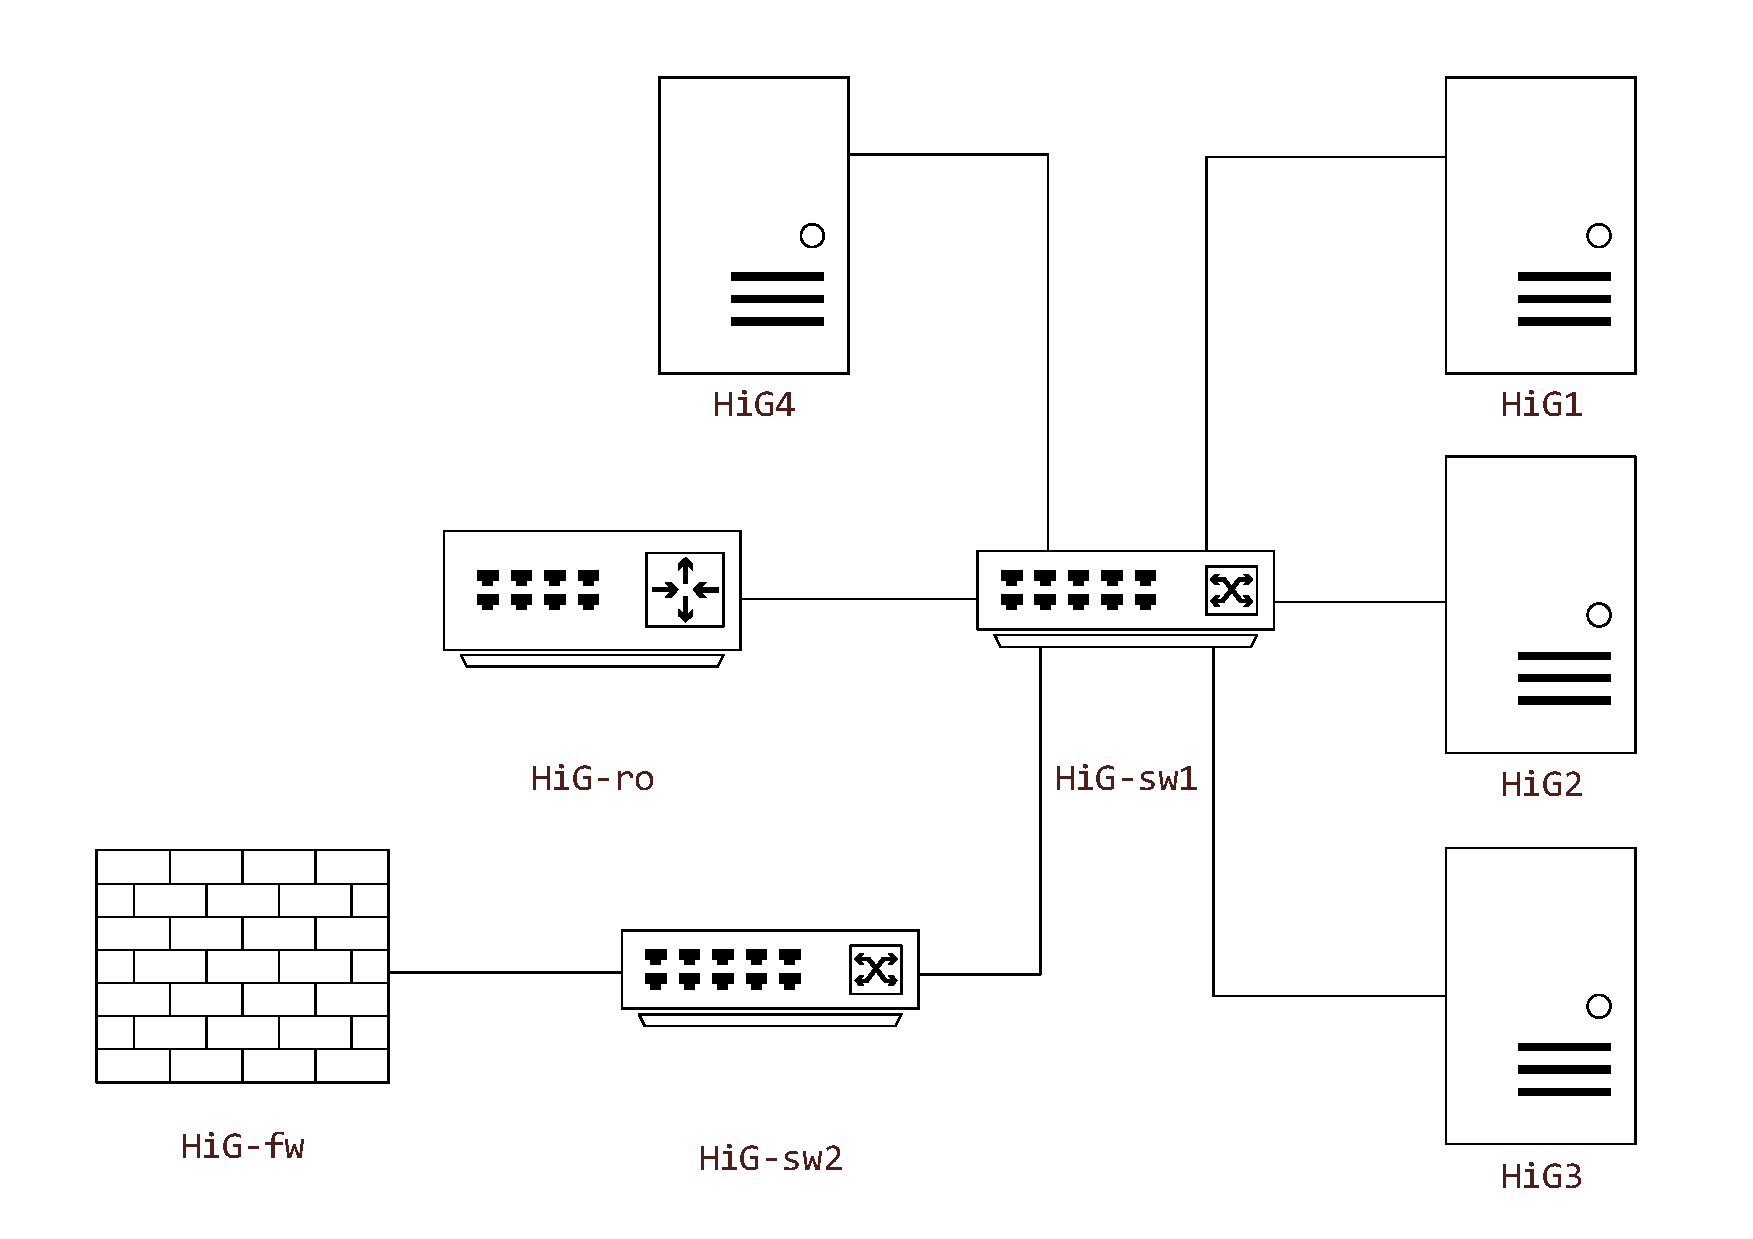
\includegraphics[scale=0.4]{img/labmiljo}
	\label{laboppsett}
    \caption{Labmiljø}
\end{figure}


\subsubsection{Produksjonsserveren}
Spesifikasjonene på bladeserveren:
\begin{itemize}
\item 4 CPU-er med 4 kjerner à 2.4 GHz
\item 32 GB RAM
\item Debian 6
\end{itemize}
Programvare:
\begin{itemize}
\item Debian 6
\item Apache2
\item MySQL
\item Icinga 1.8.4
\item SNMPtrapd
\item SNMPtt
\item Graphite
\item Metricinga 
\item sendmail
\end{itemize}

\subsubsection{Enhet for overvåkning av servermiljø}
For å overvåke temperatur og luftfuktighet på serverrommet ble det i samsvar med IKT-avdelingen kjøpt inn en APC NetBotz 200 med støtte for opptil 12 eksterne sensorer \cite{netbotz}. Denne oppfyller kravene som er gitt i oppgavebeskrivelsen. 

\section{Produksjonsserver}
"Quis custodiet ipsos custodes?" er et latinsk uttrykk som kan oversettes med "hvem passer på de som passer på?". I en overvåkningsløsning er det viktig å stille spørsmålet; hva skjer hvis overvåkningsserveren går ned? Et forslag ved starten av prosjektet var å legge overvåkningsserveren på et Xen- eller VMware-cluster. Men dette ble etter noe omtanke stemplet som en dårlig idé. Dersom clusteret gikk ned ville også overvåkningsserveren gå ned. Det ble derfor bestemt at Icinga-serveren skulle være en egen fysisk boks. 

For å sikre tilgjengeligheten til Icinga ytterligere, er det også mulig å sette opp et redundant oppsett der alle Icinga-installasjoner kan dele resultater av sjekker mellom seg. Ekstra viktig vil et slikt oppsett være dersom man knytter overvåkningssystemet mot SLA-er. Dersom en mister data om oppetid og tilgjenglighet på en tjeneste, vil en ikke lenger kunne vise hva den har vært.

En annen utfordring var å vite hvor kraftig hardware serveren trengte. Her ble referanselisten til Icinga lagt til grunn \cite{icingainaction}, hvor mange organisasjoner har lagt inn informasjon om sine oppsett. Etter avtale med oppdragsgiver ble det bestemt å sette opp en bladeserver, som eventuelt kan oppgraderes dersom det skulle bli nødvendig. 

\subsection{Installasjon}
Ved starten av iterasjonen "kjerneprogramvare" var den nyeste versjonen av Icinga 1.8.4. I pakkebrønnen for debian-stable fantes bare versjon 1.0.2 av Icinga, i backports lå 1.7.1. Icinga opprettholder en egen pakkebrønn - ``The Debian Monitoring Project'' \cite{debmon}. Fra denne kunne versjon 1.8.4 installeres. I samråd med teknisk kontakt ved IKT-avdelingen ble det bestemt å bruke versjon 1.8.4 fra debmon.

\subsubsection{Icinga Webgrensesnitt}
Webgrensesnittene "icinga-classic" og "icinga-web 1.8.1" installeres via pakkebrønnen. 

Tidlig ble det avgjort at Icinga Web skulle primært brukes som webgrensesnitt mot Icinga. Denne avgjørelsen ble tatt fordi Icinga Web har en mer moderne "look", samt bruker en Ajax Web 2.0 inspirert frontend.

Etter testing ble det oppdaget at Icinga Web inneholder feil som ble rapportert tilbake til Icinga Development Team. Feilen som ble rapportert inn omfatter søk på hostgroup-objekter eller servicegroup-objekter (link til bugreport \cite{icingawebbug}). 

Det ble derfor lagt opp til at både Icinga Classic og Icinga Web kunne benyttes på lik linje.

\subsection{Konfigurasjonsfiler}
Ved standard installasjon av Icinga er konfigurasjonen delt opp i objekttyper med flere objekter i hver fil:
\begin{itemize}
\item contacts\_icinga.cfg  
\item generic-host\_icinga.cfg     
\item hostgroups\_icinga.cfg  
\item localhost\_icinga.cfg  
\item timeperiods\_icinga.cfg
\item extinfo\_icinga.cfg   
\item generic-service\_icinga.cfg   
\item services\_icinga.cfg
\item commands.cfg
\end{itemize}
Dette var uoversiktlig og en mer oppdelt konfigurasjon var ønskelig, som også er anbefalt ved større installasjoner \cite{sysadmin} + nagios-boka. Derfor ble det bestemt å sette opp følgdende hovedinndeling (med undermapper videre der det var hensiktsmessig):

\makeatletter
\newcount\dirtree@lvl
\newcount\dirtree@plvl
\newcount\dirtree@clvl
\def\dirtree@growth{%
  \ifnum\tikznumberofcurrentchild=1\relax
  \global\advance\dirtree@plvl by 1
  \expandafter\xdef\csname dirtree@p@\the\dirtree@plvl\endcsname{\the\dirtree@lvl}
  \fi
  \global\advance\dirtree@lvl by 1\relax
  \dirtree@clvl=\dirtree@lvl
  \advance\dirtree@clvl by -\csname dirtree@p@\the\dirtree@plvl\endcsname
  \pgf@xa=0.5cm\relax
  \pgf@ya=-0.5cm\relax
  \pgf@ya=\dirtree@clvl\pgf@ya
  \pgftransformshift{\pgfqpoint{\the\pgf@xa}{\the\pgf@ya}}%
  \ifnum\tikznumberofcurrentchild=\tikznumberofchildren
  \global\advance\dirtree@plvl by -1
  \fi
}

\tikzset{
  dirtree/.style={
    growth function=\dirtree@growth,
    every node/.style={anchor=north},
    every child node/.style={anchor=west},
    edge from parent path={(\tikzparentnode\tikzparentanchor) |- (\tikzchildnode\tikzchildanchor)}
  }
}
\makeatother
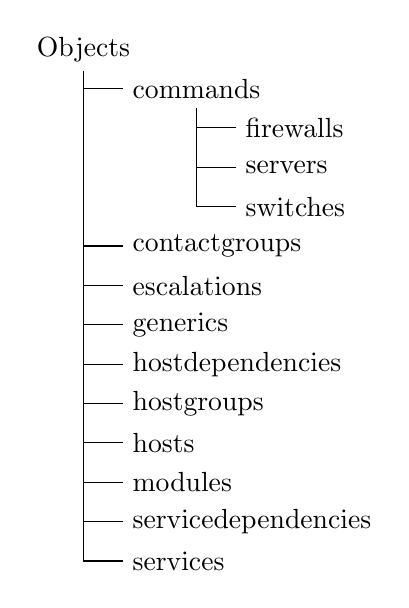
\begin{tikzpicture}[dirtree]
\node {Objects} 
    child { node {commands}
            child { node {firewalls} }
            child { node {servers} }
            child { node {switches} }
    }
    child { node {contactgroups} }
    child { node {escalations} }
    child { node {generics} }
    child { node {hostdependencies} }
    child { node {hostgroups} }
    child { node {hosts} }
    child { node {modules} }
    child { node {servicedependencies} }
    child { node {services} };
\end{tikzpicture}

Det ble testet ut et par verktøy for å administrere konfigurasjonsfilene, NConf \cite{nconf} og NagiosQL \cite{nagiosql}. Disse ble valgt bort til fordel for manuell konfigurering, da det ikke støttet oppdeling av konfigurasjon og kunne ikke kombineres med manuell konfigurasjon. I samråd med oppdragsgiver ble det avgjort av manuell konfigurasjon oppfyller kravet "Det skal være enkelt å legge til nye enheter for overvåking".

\subsection{Bruk av hostgroup}
Som nevnt i \ref{sec:objekter} knyttes et service-objekt til et host-objekt og et command-objekt for at det skal kjøres en sjekk. For å slippe å skrive et service-objekt for hvert host-objekt benyttes gruppering av host-objekter i hostgroup. Under vises et eksempel på hvordan dette er satt opp for MySQL-servere. 

Først defineres en hostgroup for alle SQL serverne. Dette gjøres for å gruppere alle SQL serverne uavhengig av hvilken databasetype som brukes. 
\begin{lstlisting}[style=example]
define hostgroup {
	hostgroup_name		sql_servers
	alias 				SQL Servers
	hostgroup_members	mysql_servers, mssql_servers, oracle_servers
}
\end{lstlisting}
Deretter defineres en hostgroup for alle MySQL-servere.
\begin{lstlisting}[style=example]
define hostgroup {
    hostgroup_name 	mysql_servers
    alias 		MySQL Servers
}
\end{lstlisting}
For å legge til en host i denne gruppen kan host-objektet være definert på følgende måte.
\begin{lstlisting}[style=example]
define host {
    use			generic_windows_host
    address		10.60.0.21
    host_name	HiG2
    alias		HiG2
    hostgroups	debian_servers, mysql_servers
}
\end{lstlisting}
Servicen som sammen med hostgroup-en og kommandoen defineres slik. Alle host-objekter i "mysql\_servers" vil da få denne sjekken.
\begin{lstlisting}[style=example]
define service {
    service_description	MySQL Connection Time
    use		 			generic_service
    name 				mysql_connection_time
    hostgroup_name 		mysql_servers
    check_command 		check_mysql_health!connection-time!0.1!0.4
}
\end{lstlisting}

Figur \ref{sql} viser en visuell fremstilling av hvordan alt dette henger sammen for alle SQL-servere:

\begin{changemargin}{-1cm}{-1cm}
\begin{figure}[H]
    \centering
    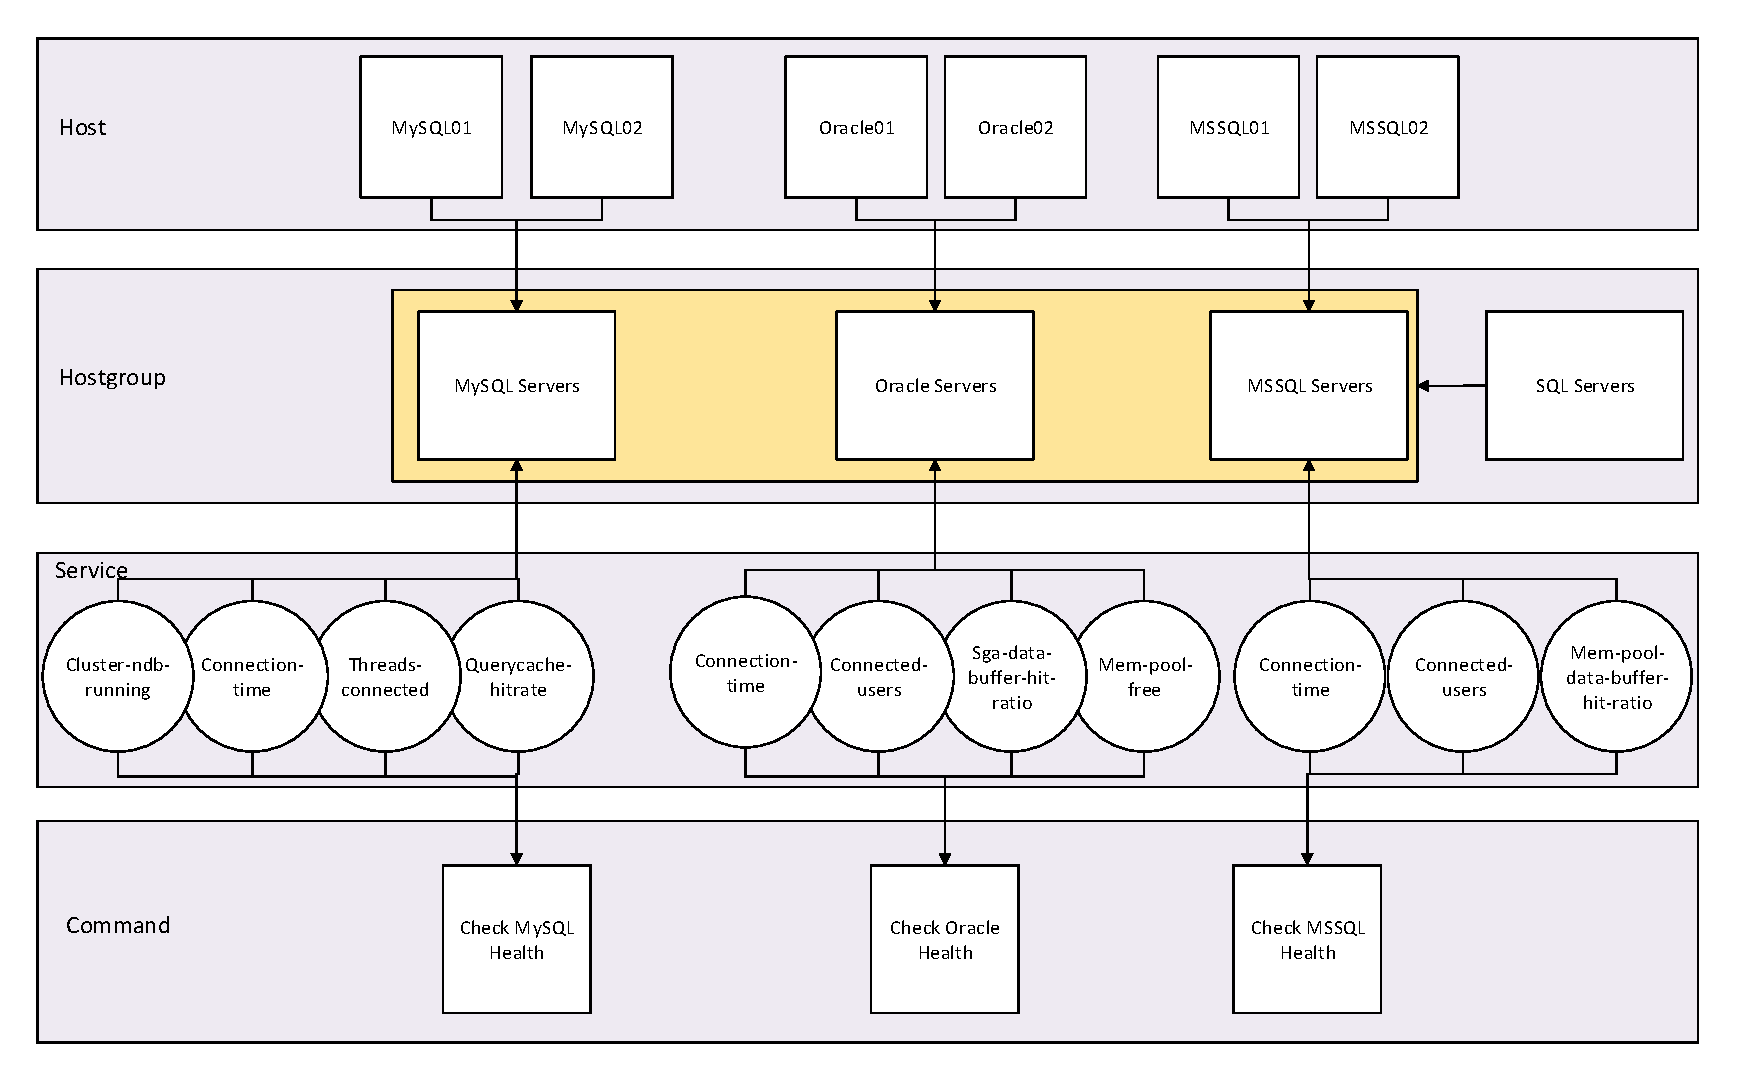
\includegraphics[scale=0.55]{img/sql}
    \caption{Visualering av konfigurasjon av SQL-servere}
    \label{sql}
\end{figure}
\end{changemargin}
\clearpage

\section{Generering av grafer}
I utgangspunktet ble det bestemt at ytelsesdata skulle holdes utenfor oppgaven. Det ble likevel satt opp en løsning for å visualisere ytelsesdata fra sjekkene med programmet Graphite\cite{graphite}. Dette ble gjort fordi det var ønskelig å kunne etablere en baseline for tjenestene slik at bedre grenseverdier kunne settes.

For å sette opp eksportering av ytelsesdataen benyttes et vanlig command-objekt i Icinga:

\begin{lstlisting}[style=example]
define command {
command_name            rotate_perf_service
    command_line            /bin/mv /usr/local/icinga/var/perfdata/service-perfdata /usr/local/icinga/var/perfdata/logs/service-perfdata.$TIMET$
}
\end{lstlisting}
 Icinga.cfg må konfigureres til å benytte dette:

\begin{lstlisting}[style=example]
process_performance_data=1
service_perfdata_file=/usr/local/icinga/var/perfdata/service-perfdata
service_perfdata_file_processing_command=rotate_perf_service
service_perfdata_file_template=[SERVICEPERFDATA]\tDATATYPE::SERVICEPERFDATA\tTIMET::$TIMET$\tHOSTNAME::$HOSTNAME$\tSERVICEDESC::$SERVICEDESC$\tSERVICEPERFDATA::$SERVICEPERFDATA$service_perfdata_file_processing_interval=200
\end{lstlisting}

For å transformere ytelsesdataene til riktig format for graphite benyttes metricinga \cite{metricinga}. Dette scriptet sjekker spool-mappen én gang i minuttet etter filer som enda ikke er prosessert og sender data inn til carbon (graphite). 
Gjennom graphite vil det dermed genereres grafer basert på ytelsesdata fra alle service-sjekker som gir dette.

Det ble også testet å modifisere scriptet til å legge outputen til service-sjekkene direkte til en MySQL-database, som vist i vedlegg /ref metricinga diff. Dette ble gjort for å oppfylle kravet fra oppgavebeskrivelsen om at alle henvendelser skal lagres i database. I samråd med oppdragsgiver ble det avgjort å gå bort i fra dette fordi det resulterte i et høyt antall nye rader over kort tid. Som et alternativ til dette kan en ta inn all data til Graphite, men aggregere det etter en viss tid. For eksempel lagre dagsgjennomsnitt for data som er eldre enn seks måneder. Dataene kan da eksporteres fra Graphite til videre bruk.

\section{Overvåkning av Windows-servere}
For overvåkning av Windows brukes NSClient++ \cite{nsclientmain}. NSClient++ er et program som brukes for å kommunisere med ulike agenter og over ulike protokoller på en ekstern server. I dette prosjektet brukes det til å hente ut informasjon via NRPE-agenten og å kjøre WMI-spørringer mot en Windows-server. NSClient++ har en konfigfil som genereres under installering. 

NSClient++ er valgt fordi klienten oppdateres hyppig \cite{nsclient}, og det er den agenten som blir referert i Icinga/Nagios dokumentasjon \cite{icingawin}. Med NSClient++ kommer også forhåndskonfigurerte plugin-er, for eksempel for å sjekke minne, CPU og harddisk.

\section{Overvåkning av Linux-servere}\label{sec:overvaklinux}
Overvåkning av standard Linux-servere skjer utelukkende ved bruk av NRPE. 

For Debian-servere kan denne installers fra pakkebrønnen "stable" med kommandoen:

\begin{lstlisting}[style=example]
apt-get install nagios-nrpe-server nagios-plugins-basic
\end{lstlisting}

For Red Hat og CentOS må det installeres en tredjeparts pakkebrønn som EPEL eller DAG før nrpe-server kan installeres med yum.

Ved bruk av DAG må en "rpm"-pakken "rpmforge" installeres for å kunne bruke pakkebrønnen, slik:

\begin{lstlisting}[style=example]
rpm -Uvh http://apt.sw.be/redhat/el6/en/x86_64/rpmforge/RPMS/rpmforge-release-0.5.2-2.el6.rf.x86_64.rpm
\end{lstlisting}

For EPEL:

\begin{lstlisting}[style=example]
sudo rpm -Uvh http://dl.fedoraproject.org/pub/epel/6/x86_64/epel-release-6-8.noarch.rpm
\end{lstlisting}

En kan verifisere at pakkebrønnene ble lagt til ved å kjøre en listing av direktivet /etc/yum.repos.d/:

\begin{lstlisting}[style=example]
$ ls -1 /etc/yum.repos.d/epel*
/etc/yum.repos.d/epel.repo
/etc/yum.repos.d/epel-testing.repo
\end{lstlisting}

Installasjon av NRPE via yum etter at pakkebrønnene er lagt til:

\begin{lstlisting}[style=example]
sudo yum install nagios-nrpe-2.12-1.el6.rf.x86_64.rpm 
\end{lstlisting}

Eksemplene er for CentOS og RHEL 6.x 64-bit.

Konfigurasjonen på Linux-servere skjer på samme måte som på Windows. Det følger ikke med noen plugin-er når en installerer nagios-nrpe-server, derfor installeres også pakken "nagios-plugins-basic".

\section{Utrulling av agenter}
NSclient++ kan lastes ned som en MSI-pakke, som kan pushes til servere med en GPO. Konfigurasjonsfilen må enten legges inn i MSI-pakken eller pushes over GPO for seg selv. Det er ikke benyttet fordi IKT-avdelingen ønsker å gjøre installasjonen manuelt, for å ha mest mulig kontroll, sikre seg mot uforutsette problemer og gjøre utrulling i faser. Det ble laget en veiledning på hvordan denne klienten skal installeres, og hvilke opsjoner som er relevant. Denne finnes i vedlegg \ref{agentguide}.

For Linux-servere installeres pakkene via pakkebehandleren, som nevnt i \ref{sec:overvaklinux}. IKT-avdelingen har bare et fåtall Linux-servere, så automatisk utrulling vil ikke være så besparende. Dersom dette skulle være ønskelig kan et enkelt script som kobler seg til og kjører kommandoen for installering skrives. Konfigurasjonsfilen kan pushes over SCP.

For annen infrastruktur brukes for det meste SNMP for å hente ut informasjon. Dette konfigureres på hver enkelt enhet, og krever vanligvis ikke noe ekstra programvare installert. I noen tilfeller brukes egne API-er for å hente ut informasjon, som for eksempel for VMware. Her må Icinga serveren ha tilgang til å bruke API-et, som vanligvis konfigureres på serveren.

\section{Lokale ressurser}
For både Linux- og Windows-servere er det satt opp noen grunnsjekker som skal kjøres på alle servere. Dette er CPU-last, harddiskplass og minnebruk. Hver sjekk er definert i et service-objekt der hostgroup-ene er satt til "windows\_servers" og "linux\_servers". 

For alle disse sjekkene er det mulig å angi grenseverdier både som prosentandel og absolutte tall. Det kan også sjekkes mot både andel ledig og andel brukt. 
\subsection{CPU}
Overvåkning av CPU vil kunne hjelpe til med å oppdage ressursproblemer. Dette kan komme av flere CPU-krevende applikasjoner på samme server eller at en applikasjon bruker all CPU-kraft.  

På Windows-servere benyttes "CheckCPU" fra NSClient++ for å sjekke CPU-last. Her legges det ved tre opsjoner i sjekken som spesifiserer tidsintervallet for datagrunnlaget, grensen for når det skal gis en advarsel og når det skal vises som en kritisk feil.

Kommandoen for pluginen slik den er definert i command-objektet. Dette henter et gjennomsnittsbruk av CPU over 5 minutter: 

\begin{lstlisting}[style=example]
./check_nrpe -u -H 10.60.0.22 -p 5666 -c CheckCPU -a time=5m warn=80 crit=90
\end{lstlisting}
Svar:
\begin{lstlisting}[style=example]
OK CPU Load ok.|'5m'=0%;80;90
\end{lstlisting}

I Figur \ref{cpuok} vises svaret fra CPU-sjekken i Icinga. 
\begin{figure}[H]
    \centering
    
\includegraphics[scale=0.8]{img/HiG3_cpu_ok}
    \caption{Visning av en OK CPU-sjekk i Icinga}
    \label{cpuok}
\end{figure}

I Figur \ref{cpucritical} ser vi at testen er kritisk på grunn av et gjennomsnittsbruk av CPU på 96 \%. 
\begin{figure}[H]
    \centering
    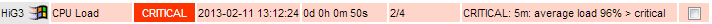
\includegraphics[scale=0.8]{img/HiG3_cpu_critical}
    \caption{Visning av en CRITICAL CPU-sjekk i Icinga}
    \label{cpucritical}
\end{figure}

I Figur \ref{cpustrain} ser vi at alle de fire CPU-kjernene jobber oppmot maksimalt. Et batch-script ble kjørt lokalt på serveren som ble overvåket for å generere CPU-bruk.

I Figur \ref{cpustrain} returnerer CPU-sjekken "OK". Dette er hentet fra gjennomsnittsbruk av CPU over 5 minutter. Like under ser vi at testen er kritisk på grunn av et gjennomsnittsbruk av CPU på 96 \%. I Figur \ref{cpustrain} ser vi at alle de fire CPU-kjernene jobber oppmot maksimalt. Et batch-script ble kjørt lokalt på serveren som ble overvåket for å generere CPU-bruk.
\begin{lstlisting}[style=example]
## winloop.bat
##
# Kjører loop.bat 10 ganger.
#
@echo off
for /l %%x in (1, 1, 10) do (
    start loop.bat
)

# loop.bat
@echo off
:loop
GOTO loop
\end{lstlisting}

\begin{figure}[H]
    \centering
    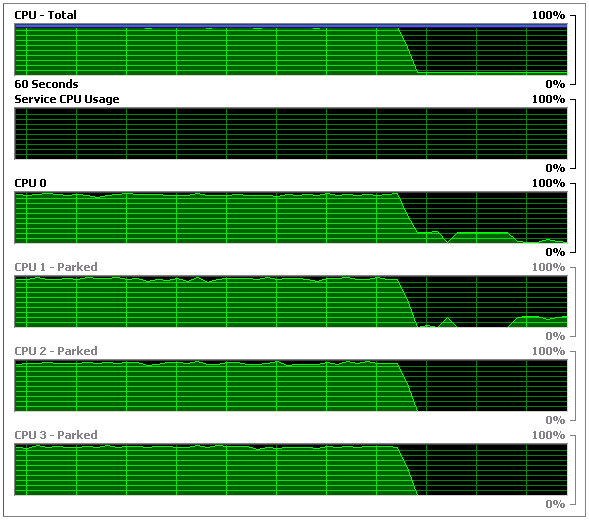
\includegraphics[scale=0.6]{img/HiG3_cpu_graph}
    \caption{CPU-bruk for HiG3}
    \label{cpustrain}
\end{figure}

På Linux-servere baserer sjekk av CPU-bruk seg på "load-average" \cite{loadavg} \cite{wiki:loadavg}. Dette er i hovedsak et gjennomsnitt for hvor mange prosesser som bruker eller venter på CPU-en, men disk- eller nettverks-I/O kan også spille inn. For maskiner med flere kjerner og/eller CPU-er vil dette fortone seg annerledes da en kan utføre flere prosesser parallelt. Load-tallene må deles på antallet CPU-kjerner for at det skal kunne brukes samme grenseverdier uavhengig av hvor mange kjerner serveren har. Dette gjøres med opsjonen "r".

Tallene som hentes ut er gjennomsnittet for de siste 1, 5 og 15 minuttene. Det er mer interessant hvis load-en er høy over lengre tid, derfor er grenseverdiene lavere for 5 og 15 minutters intervallene.
load average: 0.65 0.42 0.36

check\_load fra nagios-plugins:
I service-objektet:
\begin{lstlisting}[style=example]
check_command check_nrpe!check_dist_load!0.9,0.7,0.5 1.2,1.0,0.9
\end{lstlisting}
I konfigurasjonen på serveren som overvåkes:
\begin{lstlisting}[style=example]
command[check_dist_load]=/usr/lib/nagios/plugins/check_load -r -w $ARG1$ -c $ARG2$
\end{lstlisting}

\subsection{Minne}
Datamaskiner som bruker opp tilgjengelig minne må skrive til disk for å få plass til mellomlagrede data. Data som må hentes fra disk vil ha en betydelig høyere aksesstid enn når RAM brukes til mellomlagring \cite{wiki:mem}. 
Kontinuerlig høyt minneforbruk kan være en indikasjon på flere minnekrevende applikasjoner på samme server, en applikasjon har minnelekkasje, eller at mengden minne ikke strekker til.

*Hva en prosess kan kreve. Virtuelt minne teknologi.

For Windows-servere brukes CheckMem fra NSClient++
\begin{lstlisting}[style=example]
Check_Memory
./check_nrpe -u -H 10.60.0.22 -p 5666 -c CheckMem -a MaxWarnUsed=80% MaxCritUsed=90% type=physical
\end{lstlisting}
Svar:
\begin{lstlisting}[style=example]
OK memory within bounds.|'physical memory %'=16%;80;90 'physical memory'=1G;4;5;0;6
\end{lstlisting}

Opsjoner sendes med som gjør at sjekken gir warning når mer enn 80 \% av fysisk minne er brukt, når minneforbruket overstiger 90 \% blir minneforbruket kritisk.

For Linux benyttes plugin-en check\_mem \cite{checklinuxmem}, da det ikke følger med noen plugin for å sjekke minneforbruk i nagios-plugins.

\subsection{Disk}
En full harddisk kan skape problemer for applikasjoner som lagrer data og logger fra systemet kan stoppe. Ved høyt minneforbruk og bruk av virtuelt minne i kombinasjon med en full disk vil ikke harddisken kunne utnyttes som swap, og applikasjoner kan stoppe å fungere.

For Windows-servere benyttes "CheckDisk" fra NSClient++. For å sjekke flere disker brukes opsjonen "CHECKALL", som gir en oversikt over alle diskene på serveren.

\begin{lstlisting}[style=example]
./check_nrpe -u -H 10.60.0.22 -p 5666 -c CheckDriveSize -a Drive="C" MaxWarnUsed=90% MaxCritUsed=95%
./check_nrpe -u -H 10.60.0.22 -p 5666 -c CheckDriveSize -a MaxWarnUsed=94% MaxCritUsed=96% CheckAll
\end{lstlisting}

For Linux-servere benyttes sjekken "Check\_disk" fra nagios-plugins.
% TODO: Sjekk all mounts
Check\_Disk
\begin{lstlisting}[style=example]
./check_disk -w 8% -c 4% -e
\end{lstlisting}
Svar: 
\begin{lstlisting}[style=example]
DISK OK| /=1232MB;15430;17359;0;19288 /lib/init/rw=0MB;402;452;0;503 /dev=0MB;394;443;0;493 /dev/shm=0MB;402;452;0;503
\end{lstlisting}

\section{Tjenester}
IKT-avdelingen ønsket å overvåke tjenester og prosesser på serverne. Prossesser er instanser av programmer som kjører. Tjenester er prosesser som kjører i bakgrunnen. 

Overvåkning av tjenester vil innebære å se på om en eller flere prosesser kjører til en hver tid. NSClient++ har muligheten til å se om en bestemt prosess eller tjeneste kjører eller har stoppet gjennom CheckServiceState. Her spesifiserers navnet på prosessen eller tjenesten, og sjekken svarer på om denne finnes i prosesstabellen.
\begin{lstlisting}[style=example]
define service {
    service_description     DHCP Service
    hostgroup_name          dhcp_servers
    check_command           check_nrpe!CheckServiceState!DHCPServer=started ShowAll
    use                     generic_service
}
\end{lstlisting}
Linux-plugin fra nagios-plugins: check\_procs. Her spesifiseres også hvor mange instanser av prosessen som skal forekomme. 
\begin{lstlisting}[style=example]
define service {
    use            	        generic_service
    hostgroup_name       	linux_servers
    service_description     NRPE Check my process
    check_command        	check_nrpe!check_process!sshd 1:40
}
\end{lstlisting}

Å se at en tjeneste kjører via Windows kan gi falsk informasjon. Et eksempel her er Microsofts terminal services. Tjenesten står som kjørende i Windows, men brukere får ikke koblet til. Dette kommer av at tjenesten har hengt seg, uten at den står som "stoppet". Dette merkes ikke før brukere ringer inn og beskriver problemet \cite{serviceproblem}. Som nevnt i \ref{sec:omovervakning} vil en bedre sjekk være å teste selve tjenesten, som blir gjort for tjenestene beskrevet under.

\subsection{LDAP, DNS og DHCP}
Tjenester som LDAP-autentisering, DNS-oppslag og DHCP-leasing er en viktig del av tjenestene IKT-avdelingen leverer.

LDAP-tjenesten gjør at brukere får logget på trådløse nettverk og autentisert seg for andre tjenester IKT-avdelingen leverer \cite{ldap}.

DNS-oppslag gjøres hver gang en enhet skal oversette en IP-adresse til et hostname eller omvendt. Uten DNS vil ikke enheten kunne kontakte andre enheter ved å benytte hostname, som brukes i eksempelvis web-adresser \cite{dns}. 

Når en ny enhet kobles til nettverket vil denne få tildelt en IP-adresse av DHCP-serveren. Samtidig får den informasjon om gateway og DNS-servere. Uten dette vil ikke enheten få kommunisert med andre enheter på nettverket \cite{dhcp}.

Sjekkene for alle de tre tjenestene vil bli gjort direkte fra Icinga-serveren. Denne står i et eget nettverk. Derfor vil det kunne oppstå situasjoner der Icinga rapporterer at tjenestene fungerer, men det ikke fungerer for brukere tilkoblet andre nettverk. En løsning på dette kan være å kjøre sjekkene via en server i hvert nettverk brukere er tilkoblet.

\subsubsection*{LDAP}
For å overvåke LDAP-tjenestene benyttes pluginen "check\_ldap" som følger med i nagios-plugins. Plugin-en kobler til LDAP-tjenesten og prøver å autentisere en spesifisert bruker. Her vil sjekken returnere OK, om den fikk autentisert. 

Ytelsesdata har blitt samlet inn for å sette grenseverdier for når Icinga skal gi varsel om treg innlogging. I Figur \ref{ldapauth-inv} vises det at tjenesten sjekket på fire LDAP-servere, over en måneds periode bruker rundt 0.0044 sekunder på å autentisere. Ut ifra dataen som er samlet inn settes grenseverdien for WARNING til 0.01 sekund, og CRITICAL til 0.02 sekunder.

\begin{figure}[H]
    \centering
    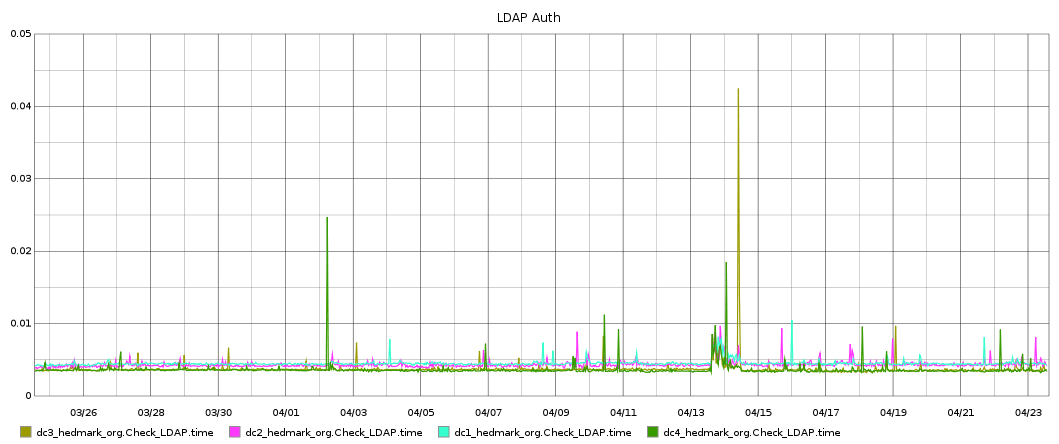
\includegraphics[width=1.0\textwidth]{img/ldap-auth-inv}
    \caption{Data fra Graphite (sekund)}
    \label{ldapauth-inv}
\end{figure}

\subsubsection*{DNS}

DNS overvåkes med plugin-en "check\_dns". Denne, på samme måte som "check\_ldap" kobler seg til selve tjenesten. Dette fungerer ved å gjøre et DNS-oppslag på en spesifikk IP-adresse, og verifisere dette mot et satt hostname. Dersom dette stemmer vil plugin-en returnere OK, sammen med ytelses-data på hvor lang tid oppslaget tok.

Figur \ref{dns-inv} viser data samlet inn fra to DNS servere over 30 dager. Disse dataene viser forventet tid for et oppslag, og ut ifra dette ble grenseverdien for WARNING satt til 0.01 sek og CRITICAL til 0.02 sek.

\begin{figure}[H]
    \centering
    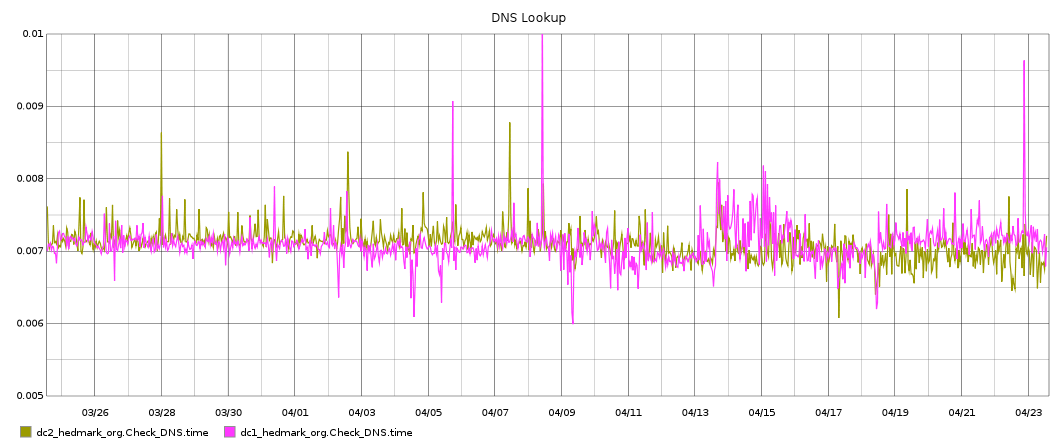
\includegraphics[width=1.0\textwidth]{img/dns-inv}
    \caption{Data fra Graphite (sekund)}
    \label{dns-inv}
\end{figure}

\subsubsection*{DHCP}
DHCP tjenesten overvåkes med pluginen "check\_dhcp". Denne sender en DHCPDISCOVER-pakke til DHCP-serveren. Hvis DHCP-tjenesten fungerer får pluginen en DHCPOFFER-pakke som respons. Dersom denne inneholder en korrekt lease, returnerer pluginen OK til Icinga sammen med tiden det tok.

\subsection{Terminal Services(Counters)}
Mange interne applikasjoner kjøres via terminalservere. Det er det viktig at terminalserverne er stabile fordi hver enkelt brukes som en lokal maskin av mange brukerne. Ofte kan terminalservere belastes mer i perioder, derfor overvåkes hvor mange aktive brukere som er tilkoblet. Da kan en se hvilke som er belasted mest og når det er behov for å sette inn flere servere.

Antallet aktive og inaktive brukere kan hentes ut fra Windows Performance Counters direkte. Dette kan sjekkes gjennom NRPE og NSClient++. I Figur \ref{ts-skole-usage} er bruken for en uke samlet inn. Ut ifra bruken over en måned er WARNING og CRITICAL satt til 25 og 35 for å varsle unormal bruk.

Kommando som er brukt for å sjekke antallet aktive brukere på en terminalserver er:
 
\begin{lstlisting}[style=example]
	command_line	check_nrpe -u -H $HOSTADDRESS$ -p 5666 -c CheckCounter -a "Counter:Active=\\Terminal Services\\Active Sessions" ShowAll MaxWarn=25 MaxCrit=35
\end{lstlisting}

\begin{figure}[H]
	\centering
	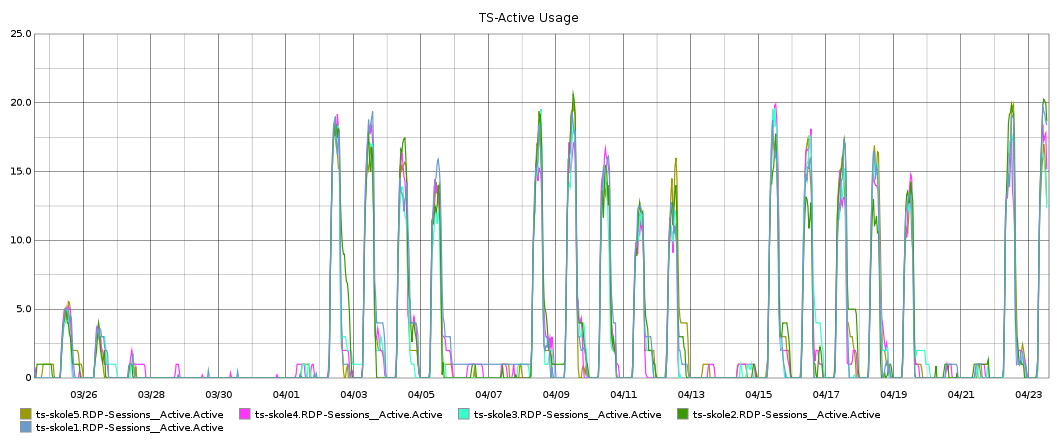
\includegraphics[width=1.0\textwidth]{img/ts-skole-usage-inv}
	\caption{Data fra Graphite (Antall)}
	\label{ts-skole-usage}
\end{figure}

\subsection{Webservere}
IKT-avdelingen drifter mange webservere som benyttes av, eller gir informasjon til brukere. Pluginen "check\_http" \cite{checkhttp} fra nagios-plugins benyttes for å sjekke at tilkoblingen til webserveren svarer på henvendelsen. Deler av forventet innhold sjekkes for å se at websiden ikke har blitt endret av uvedkommende.

Kommandoen for å gjøre dette er for siden http://portal.hedmark.org:
\begin{lstlisting}[style=example]
./check_http -H portal.hedmark.org -s "Velkommen til Hedmark fylkeskommunes portal" -S 
\end{lstlisting}

For websider som skal svare på HTTPS sjekkes også utløpsdato for SSL-sertifikatet. I eksempelet under vil plugin-en gi en WARNING om sertifikatet utløper innen 50 dager:
\begin{lstlisting}[style=example]
./check_http -H portal.hedmark.org -C 50
\end{lstlisting}

\subsection{Redundante oppsett}
En ordinær plugin henter status for en service på ett host-objekt. Ved redundante oppsett vil det ikke nødvendigvis være kritisk om en av nodene er nede. For å vurdere statusen av et cluster kan en kjøre en sjekk på hvert enkelt host-objekt, og ta en vurdering basert på resultatene av alle sjekkene samlet.

For å overvåke redundante oppsett, har plugin-ene check\_multi \cite{checkmulti} og check\_cluster \cite{checkcluster} blitt vurdert. Forskjellene på disse er at check\_cluster parser den lokale status.dat filen og ser hvilken tilstand en service eller en host er ved siste sjekk. Pluginen check\_multi derimot kjører plugin-er mot spesifiserte host-objekter, og en kan definere sammenligningsoperator (<,>,=), som vil bli sjekket mot de returnerte resultatene.

Med check\_multi kan en benytte en eller flere egendefinerte kommandoer som parametere. Disse vil parses av check\_multi og kan inneholde alt i fra "echo 'Hello, World!'", til mer avanserte Perl-script som kjøres ved hjelp av eval. For å evaluere resultatene kan en definere kriterier som gir et varsel (her brukes standard Icinga-tilstander). 

Eksempel:
\begin{lstlisting}[style=example]
command [ HTTP_Node1 ] = check_http -H 192.168.2.10
command [ HTTP_Node2 ] = check_http -H 192.168.2.11
command [ HTTP_Node3 ] = check_http -H 192.168.2.12
state [ WARNING ] = COUNT(WARNING) > 2
state [ CRITICAL ] = COUNT(CRITICAL) > 3
\end{lstlisting}
For check\_cluster spesiferes det om det er et host- eller service-cluster en skal sjekke. Deretter spesifiseres parametere med navn på host og service, og hvor mange hosts eller services som må være nede før at det skal varsles med WARNING eller CRITICAL. Siden check\_cluster kjører lokalt på Icinga-serveren vil den ikke bruke noe nettverkstrafikk, noe som er positivt. Ulempen er at den ikke gir noen informasjon om hvilket host-objekt som er nede eller hvilket host-objekt en service feilet på. Det vil si at den gir bare en overordnet status for det redundante oppsettet     

Under vises et eksempel hvor servicen Check HTTP for host-objektene localhost, HiG2, HiG3, og HiG4 blir kjørt og vil gi WARNING om en av dem er nede og CRITICAL om to av dem er nede: 
\begin{lstlisting}[style=example]
check_cluster --service -l "Check HTTP"  -d $SERVICESTATEID:localhost:Check HTTP$, $SERVICESTATEID:HiG2:Check HTTP$ ,$SERVICESTATEID:HiG4:Check HTTP$  -w @1 -c @2
\end{lstlisting}

\subsection{Microsoft Exchange}

Microsoft Exchange benyttes som e-postsystem for fylkeskommunen. Her routes og lagres all e-post som sendes ut og inn av alle brukere. I tillegg benyttes kalenderfunksjonalitet. Exchange er kritisk for kommunikasjon mellom ulike avdelinger i fylkeskommunen og utdad. 

Som for terminalservere, beskrevet i \ref{sect:Terminalservere}, brukes Microsoft Performance Monitor for å få tilgang til en rekke viktige tall om Exchange-serverenes ytelse. Disse overvåkes over NRPE med check\_counter i NSClient++. Firmaet SolarWinds, som selger en kommersiell overvåkningsløsning anbefaler blant annet at følgende parametre overvåkes\cite{exchange}:
\begin{itemize}
	\item Antall tilkoblinger. Dersom antallet er høyt kan det føre til at e-postklienter oppfattes som trege av brukerne.
	\item Gjennomsnittlig responstid på forespørsler. Høye tall vil oppfattes som treghet for brukerne.
	\item Antall meldinger sendt per sekund. Ved høye tall kan det være mistanke om at mail-serveren blir brukt til spam, eller at klienter på nettverket har blit kompromittert.
	\item Antall LDAP-søk som gir timeout. Høye tall kan indikerer mange tilkoblingsfeil mot Active Directory.
	\item Størrelse på leveringskø. Antall meldinger som venter på å bli prosessert.
\end{itemize}
Microsoft har gitt ut egne anbefalinger til grenseverdier som er benyttet som et utgangspunkt\cite{exchangethresholds}.

I tillegg til disse var det ønskelig med en sjekk som testet hele e-post-oppsettet. Til dette benyttes pluginen "check\_email\_delivery" \cite{exchange}. Her sjekkes det at en e-post kan sendes fra SMTP-serveren. E-posten som sendes ut inneholder en unik ID. Videre kobler pluginen seg til IMAP-tjenesten og sjekker om e-posten med den unike ID-en kom frem. Antall sekunder for hele round-tripen blir målt. Helst skulle en sendt e-posten fra en SMTP-server som står utenfor nettverket, men det var ikke tilgjengelig under implementasjonen.

Det sjekkes også at websiden for Outlook Web Access er tilgjengelig, på samme måte som andre websider, slik det er beskrevet i \ref{Webservere}.
\section{Databaser}
Tre forskjellige databasemotorer benyttes av IKT-avdelingen. Disse er MySQL, MSSQL og Oracle DB. Disse har ulik arkitektur og virkemåte \cite{databasecomparison}, og derfor blir ikke de samme parameterne overvåket på alle. Felles for alle er:

\begin{itemize}
	\item Connection time (tid det tar å koble til SQL serveren).
	\item Connected users (antall aktive sessioner mot SQL serveren).
	\item Cache hit rate (antall spørringer som blir hentet fra cache i et tidsintervall).
\end{itemize}

Disse sjekke er spesifikke for hver databasemotor, og er valgt for å få en oversikt over trege spørringer som utføre.

\begin{itemize}
\item MySQL: Slow queries (antall trege spørringer SQL serveren utfører i et tidsintervall).
\item MSSQL: Lazy writes ()
\item Oracle: Free table space (Plass ledig for tabellene).
\item Oracle: Switch interval (Overvåker load).
\end{itemize}

\subsection*{Connection time}
Connection time gir beskjed dersom det ikke er mulig å koble til SQL-serveren. Hvis denne sjekken gir en timeout, er det fordi sjekken ikke får kontakt på porten til serveren. Her definerers det parametere for hvor lang tid det bør ta å koble til. Hvis tilkoblingstiden blir for lang varsler Icinga om dette. Grenseverdier her er valgt ut fra gjennomsnittlig tilkoblingstid over 30 dager.

\subsection*{Connected users}
Connected users sjekker hvor mange sessioner som er koblet til database tjenesten (per instanse for Oracle DB). Antall aktive sesjoner blir samlet inn om hver enkelt database. Derfor defineres grenseverdier ut fra hvor mange brukere som er koblet til over en periode. Da plukkes uvanlige bruksmøstre opp og kan videre studeres.

\subsection*{Cache hit}
Cache hit er hvor ofte data hentes ut fra databasemotorens egen cache, slik at dataen ikke leses fra disk. Dette sparer diskene for I/O-operasjoner. Hvis cache hit ligger på et høyt nivå (90-100 \%), indikerer dette at tabellene det spørres mest mot lagres i cache. Når cache hit ligger under 90 \% kan dette være et resultat av at serveren ikke har nok minne til å lagre tabellene i cache. Dette kan indikere et minneproblem.

Oracle mener at cache hit bør ligge på over 90 \% \cite{oraclecachehit}. For MSSQL er tilnærmet 100 \% cache hit et godt utgangspunkt \cite{sqlmonitoring}.

MySQL-databasene til IKT-avdelingen lagrer all databasedata i minnet, så her vil det ikke være relevant å sjekke cache hit. Sjekken er satt opp slik at ordinære MySQL-servere vil kunne settes opp med denne sjekken i ettertid.

%\subsection{Plugin} %???
For at Icinga-serveren skal kunne snakke med de forskjellige databasemotorene trengs en klient for hver av dem. 

\subsubsection{Oracle}
Databaseklienten finnes på Oracle sine nettsider \cite{oracleclient}. Den finnes ikke som en deb-pakke, som som brukes for Debian. Det finnes derimot en rpm-pakke, som brukes av blant annet Red Hat. Alien ble brukt til å konvertere rpm-pakken over til deb-pakke før installasjon på Icinga-serveren \cite{debian:alien}. 

\begin{lstlisting}[style=example]
alien oracle-instantclient11.2-basic-11.2.0.3.0-1.x86_64.rpm 
dpkg -i oracle-instantclient11.2-basic-11.2.0.3.0-1.x86_64.deb
\end{lstlisting}

Da denne er installert kreves følgende miljøvariable for at klienten skal fungere, og finne tnsnames filen.
Disse må legges til i environment variablene til Icinga for at "nagios-brukeren" skal få tilgang.
% need config

\begin{lstlisting}[style=example]
export ORACLE_HOME=/usr/lib/oracle/11.2/client
export TNS_ADMIN=/usr/lib/oracle/11.2/client/network/admin
\end{lstlisting}

Videre trengs også en databasedriver, som gjør det mulig for Perl å benytte klienten. For Oracle-databaser brukes "libdbd-oracle-perl".

På en Oracle-server vil hver database ha sin egen instans \cite{oraclefaq}. Derfor vil parametere som overvåkes være forskjellig fra database til database. Navnene til instansene legges derfor inn som en egendefinert variabel i hver enkel Oracle-servers host-objekt. Når plugin-en kjøres sjekkes filen tnsnames.ora, som inneholder tilkoblingsinformasjon for hver enkelt instans. Strukturen på tnsnames.ora vises under:

\begin{lstlisting}[style=example]
ORA11 =
 (DESCRIPTION = 
   (ADDRESS_LIST =
     (ADDRESS = (PROTOCOL = TCP)(HOST = 127.0.0.1)(PORT = 1521))
   )
 (CONNECT_DATA =
   (SERVICE_NAME = ORA11)
 )
)
\end{lstlisting}

Check\_multi brukes for å samle en Oracle-servers instanser under samme service-objekt. For eksempel når cache hit-sjekken kjøres, vil check\_multi utføre sjekken for alle instansene. I webgrensesnittet vil svarene fra instansene samles under "check cache hit" for hvert enkelt host-objekt. Dette gjør det mer oversiktlig og dynamisk enn en sjekk for hver instans. Under vises konfigurasjonen for dette.

\begin{lstlisting}[style=example]
define service {
...
    check_command check_multi!check_oracle! -s dbinstances=$_HOSTDBINSTANCES$ -s host=$HOSTADDRESS$ -s mode=sga-data-buffer-hit-ratio -s warning=93: -s critical=90: -s user=$USER5$ -s pass=$USER4$
}

define command {
...
	command_line	check_multi -r 32 -f /etc/icinga/objects/commands/check_multi/$ARG1$.cmd $ARG2$
}
\end{lstlisting}
%TODO: EXPLAIN
\begin{lstlisting}[style=example]
eeval [ oracle_health ] =
    my $chain = "";
    foreach my $instance (split(/,/,'$dbinstances$')) {
        $chain .= "-x \"command[ $instance ] = check_oracle_health --connect '$user$'\/'$pass$'\@'$instance' --mode '$mode$' --warning $warning$ --critical $critical$ \" ";
    }
    parse_lines("command [ check_oracle ] = check_multi -r 4 $chain");
\end{lstlisting}


\subsubsection{MySQL}
For MySQL ligger de nødvendige pakkene i Debians pakkebrønn og kan installeres med apt. De nødvendige pakkene er "mysql-client", for databasetilkoblingen og "libclass-dbi-mysql-perl", som er en Perl-modul for å kunne koble til en MySQL-server.

\subsubsection{MSSQL}
For MSSQL var det vanskelig å finne en databaseklient som er fri programvare. Her endte vi opp med FreeTDS \cite{freetds}, sammen med Perl-modulen "libdbd-sybase-perl".

\subsection{Plugin}
Plugin-ene som blir benyttet for databaser er skrevet av firmaet "Consulting \& Solutions" og heter "Check\_MySQL\_Health", "Check\_Oracle\_Health" og "Check\_MSSQL\_Health" \cite{consol}.

Disse må kompileres fra kildekoden. For å gjøre dette må en først konfigurere de med riktige parametere. Dette er de samme for alle tre plugin-ene.

\begin{lstlisting}[style=example]
./configure --prefix=/usr/lib/nagios/plugins/ --with-nagios-user=nagios --with-nagios-group=nagios --with-perl=/usr/bin/perl --with-statefiles-dir=/tmp
\end{lstlisting}

Plugin-en kompileres og legges i riktig bane ved å kjøre kommandoene

make\\make INSTALL

For å koble til databaseserverne trengs servicebrukere i hver av de. Her holder det med minimale tilganger slik at denne ikke har tilgang til å endre tabeller og spørre etter info. Brukeren vil kun ha tilgang til å kjøre "Server administrasjon" kommandoer \cite{mysqlpriv}.

I MySQL brukes følgende kode for å opprette denne brukeren:
\begin{lstlisting}[language=SQL,style=example]
GRANT USAGE ON *.* TO 'icinga'@'10.60.0.20' IDENTIFIED BY 'Password';
\end{lstlisting}

Script for å opprette brukere i Oracle og MSSQL finnes i Vedlegg \ref{oracledb.sql} og \ref{mssqldb.sql}.

Konfigurasjonen
Kommandoen konfigureres med muligheten for å bestemme hvilken sjekk som skal kjøre i \$ARG1\$.

Her brukes MySQL som eksempel, men dette vil være likt for de to andre SQL serverne. 
\begin{lstlisting}[style=example]
    command_line $USER1$/check_truedatabase-motor>_health --hostname=$HOSTADDRESS$ --username=$USER5$ --password=$USER4$ --mode $ARG1$ --warning $ARG2$ --critical $ARG3$
\end{lstlisting}

\subsubsection{MySQL Cluster}

MySQL Cluster er et distribuert oppsett for MySQL. Ved IKT-avdelingen benyttes et MySQL Cluster med NDB som lagringsmotor, der databasene kjører i minnet. Et MySQL Cluster består av tre forskjellige nodetyper \cite{ndbinformation}:

\begin{itemize}
	\item Management - her konfigureres clusteret og en setter opp hvor mange Data- og SQL-noder som kan kobles til.
	\item Data - oppbevarer tabeller og tabelldata i RAM. Disse håndterer lastbalansering, replikering, failover og gjenoppbygging automatisk i mellom hverandre.
	\item SQL - MySQL servere som kobler seg til data-nodene for å hente og lagre data.
\end{itemize}


Den enkleste måten å hente ut statistikk for et MySQL Cluster, er å benytte administrasjonsprogrammet "ndb\_adm". Denne kan hentes ut fra installasjonspakken til mysql-cluster \cite{ndbdownload}. I ndb\_adm kan en se hvor mange noder av hver type som er tilkoblet management-noden og minneforbruket til hver av datanodene. De plugin-ene som benyttes baserer seg på output fra "ndb\_adm".

Antallet noder tilkoblet overvåkes med pluginen check\_ndbd \cite{ndbnode}. Her ble det gjort en endring i koden slik at serveren som ndb\_adm kobler seg til kan spesifiseres som en parameter.

For minnebruk ble det skrevet en egen plugin, da ingen eksisterende plugin ble funnet som tillater å spesifisere hvilke noder som skal sjekkes. ID-ene til nodene som skal sjekkes ble satt opp som en egendefinert variabel i host-konfigurasjonen. Denne sendes til pluginen via service- og kommando-objektene. Konfigurasjonen for dette er vist under.

\begin{lstlisting}[style=example]
define host {
	...
	_NODEIDS 2,3  ;Data-nodes IDs to check memory usage
}

define command {
	...
	command_line   $USER1$/libexec/check_ndb_mem.pl --host $HOSTADDRESS$ --nodes $ARG1$ --warning $ARG2$ --critical $ARG3$
}
\end{lstlisting}
\section{Applikasjoner}
Muligheten for å se om en applikasjon fungerer slik den skal, er en viktig del av overvåkningen. Det er applikasjonene brukerne benytter seg av og vil sende inn feilmeldinger om. En applikasjons tilstand vil bestemmes av flere tjenesters status. I Icinga benyttes et servicegroup-objekt for å gruppere flere service-objekter.

Et praktisk eksempel på dette vises i Figur \ref{servicegroup_layout}. Her vil applikasjonen "Web App for ERP" være avhengig av webserveren for å vise web-grensesnittet til brukerne. En filserver for lesing og lagring av filer, en e-post-server for å sende og motta e-post og en databaseserver som inneholder brukerinfo og andre tabeller. 

\begin{figure}[H]
    \centering
    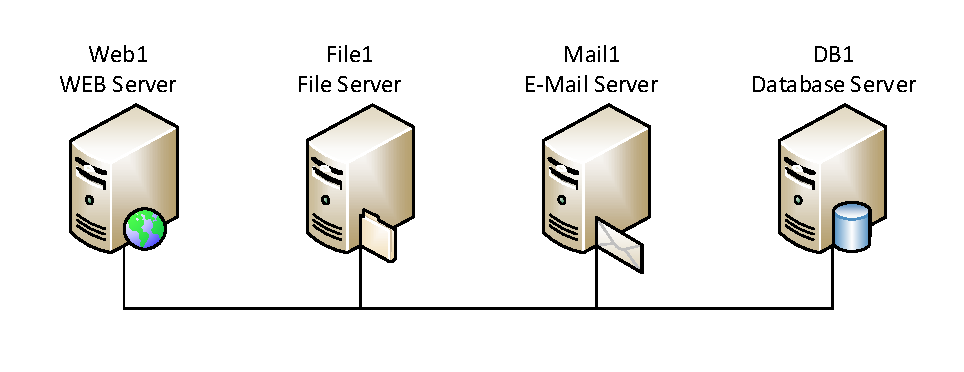
\includegraphics[scale=0.6]{img/servicegroup_layout}
    \caption{Tjenester for servicegroup-objektet ERP\_WEBAPP}
    \label{servicegroup_layout}
\end{figure}

Konfigurasjonen for dette er vist under. Direktivet "Members" setter medlemmene i gruppen der hvert service-objekt er "host\_name,service\_description".

\begin{lstlisting}[style=example]
define servicegroup {
	servicegroup_name ERP_WEBAPP
	alias Web App for ERP
	members Web1,Check HTTP, File1,Check SMB, Mail1,Check Exchange, DB1,Check MySQL
}
\end{lstlisting}

Her kjøres service-sjekker mot alle tjenestene. Service-objektene grupperes i en servicegroup. Dette gjør at vi får et oversiktsbilde over applikasjonen i Icingas web-grensesnitt som vist i Figur \ref{servicegroup_web}. Slik blir det enklere for servicedesk å kunne gå inn og se hva som er feil med "Web app for ERP" om brukere rapporterer om feil på denne applikasjonen.

\begin{figure}[H]
    \centering
    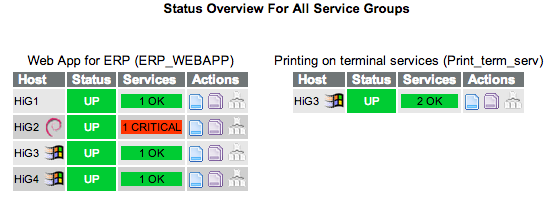
\includegraphics[scale=0.6]{img/servicegroup_web}
    \caption{ Oversikt over servicegroup-objekt og status i webgrensesnittet}
    \label{servicegroup_web}
\end{figure}

Det vil det også være naturlig å sette opp servicedependency-er mellom ERP Web1 og sjekkene for webserveren, filserveren, mailserveren og databaseserveren.

\section{Infrastruktur}
Infrastruktur består av de grunnleggende enhetene de andre serverne er avhengig av. I dette prosjektet er det definert til: switcher, routere, brannmurer, UPS, virtualiseringsteknologi og serverrommiljø.

Infrastrukturovervåkning er essensielt for å kunne levere IT-tjenester. Det er viktig at design av overvåkningen fører til at man raskt og effektivt skal kunne oppdage og presentere feil som oppstår. For å få til dette i Icinga benyttes "parent" \ref{sec:parents}. De aller fleste enheter i infrastrukturen (untatt servermiljø) vil være parent for andre enheter. Dette reflekteres i et statuskart i Icinga, som vist i Figur \ref{statusmap}.

\subsection{Switcher}\label{sec:switch}
Switcher er nettverksutstyr som jobber på lag 2 i OSI-modellen, datalink-laget. IKT-avdelingen benytter switcher med lag 3-funksjonalitet. Det vil si at switchen kan kommunisere over IP. Alle switchene IKT-avdelingen benytter støtter SNMP-protokollen, som brukes til overvåkingen.

På switchene overvåkes forskjellige sensorer avhengig av hvilke som finnes. Alle switcher har for eksempel ikke vifter.

Det er laget et generisk oppsett som overvåker temperatur, PSU og viftestatus. Hvilken OiD denne informasjonen ligger under varierer fra leverandør til leverandør. For noen produsenter kan denne også være lik. 

Dersom en vifte eller PSU rapporteres som defekt vil det rapporteres som en CRITICAL-status i Icinga. For temperatur er grenseverdiene satt til xx for WARNING og xx for CRITICAL.

Switchene IKT-Avdelingen bruker er forskjellige modeller fra leverandørne Cisco, Dell og HP. Disse overvåkes med plugin-ene "check\_nwc\_health" \cite{checknwc} for Cisco og HP, og check\_snmp\_powerconnect for Dell \cite{checkpowerconnect}.

\subsection{Routere og brannmurer}
IKT-avdelingen benytter Cisco ASA- og Cisco PIX-routere for routing av trafikk mellom forskjellige nettverk. I tillegg utfører de oppgaver som pakkefiltrering, NAT og IPsec-tunneler.
% TODO: Sjekk at dette er riktig mot docs

\subsubsection{Ressurser}
Som for switcher brukes check\_nwc\_health til å se at sensorer er OK. I tillegg sjekkes CPU-bruk og minneforbruk gjennom samme plugin. 

For CPU-bruk sjekkes gjennomsnittet over 5 minutter. Grenseverdier er satt til 80 \% på WARNING og 90 \% på CRITICAL, i henhold til det Cisco anbefaler \cite{ciscounifiedcommunication}. Høy CPU-bruk kan føre til dårligere ytelse, høy rate av buffer-feil og generelle feil med responsivitet \cite{ciscocpurouters}

I følge Cisco kan høyt minneforbruk under vanlig drift indikere at brannmuren er under angrep. \cite{ciscomem}. Dersom en router bruker opp tilgjengelig minne kan det føre til at routeren slutter å svare på kommandoer, telnet-tilkoblinger eller henger \cite{ciscomemproblem} . Cisco anbefaler en grenseverdi på 15 \% ledig minne \cite{ciscounifiedcommunication}. Grenseverdier for minne er derfor satt til 20 \% for WARNING og 15 \% for CRITICAL.

\subsubsection{Failover}
Cisco-routere og brannmurer har en viktig funksjon som kalles failover. Failover fungerer ved at to like enheter settes opp, der en blir satt som "primary" og den andre som "secondary". Secondary kan da overta for primary dersom det skulle bli nødvendig. Routerne kobles sammen med en seriellkabel. Figur \ref{ciscoasafailover} viser oppkoblingen for et Cisco-failover-oppsett. 

\begin{figure}[H]
    \centering
    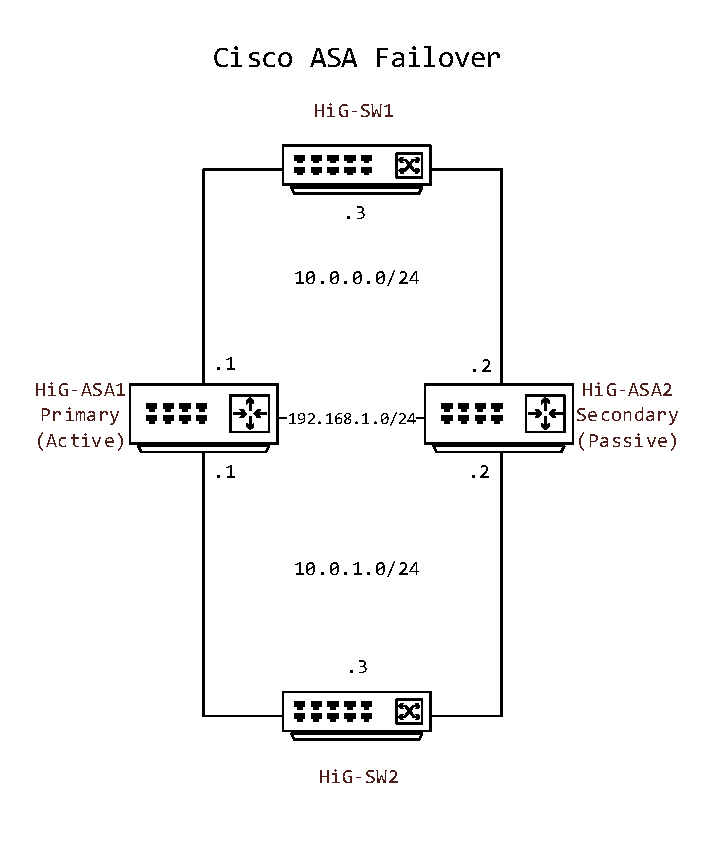
\includegraphics[scale=0.6]{img/asafailover}
    \caption{Oppsett for Cisco-failover}
    \label{ciscoasafailover}
\end{figure}

Dersom primary går ned, vil secondary ta over nødvendige ruter, brannmurregler og konfigurasjon. Secondary vil dermed overta IP- og MAC-adressen til primary. Primary vil bli satt som passiv (trenger ikke nødvendigvis å ha en passiv IP-adresse, fordi IP-kommunikasjon kun går gjennom det aktive interfacet) helt til en manuelt endrer dette tilbake i konfigurasjonen. \cite{ciscofailover}. 

Sjekkene som settes opp for å verifisere at failover-funksjonaliteten fungerer som den skal, og at det ikke har intruffet feil er:
\begin{itemize}
\item Hvis primary er satt som aktivt og secondary er passiv returneres OK.
\item Om primary er satt som passiv returneres WARNING. 
\item Om secondary er satt som aktiv returneres WARNING.
\item Hvis primary eller secondary får en error returneres CRITICAL.
\item Hvis failover ikke er konfigurert returneres UNKNOWN. 
\end{itemize}

Til dette benyttes plugin-en "check\_cisco\_firewall" \cite{checkciscofirewall}.

Hvis brannmurene deler management IP på primary og secondary, er det ingen mulighet for å hente ut informasjon fra den passive brannmuren. Da sjekkes failover status bare for primary. I et ideelt miljø bør både passiv og aktiv enhet ha hver sin IP-adresse, slik at fysiske feil også kan avdekkes på den passive.

Begge brannmurene legges i en hostgroup som er lagt på service-objektet for "cisco\_health", slik at lokale ressurser sjekkes på samme måte som switcher. Brannmurene legges også inn i en hostgroup som heter Cisco-failover som benyttes i service-objektet for failover.

\subsubsection{VPN}
For brannmurer som har VPN-tjeneste sjekkes antall oppkoblede brukere opp mot det antallet brannmuren er lisensiert for. Begge disse verdiene finnes som SNMP OID-er definert i "CISCO-FIREWALL-MIB" \cite{cisco_fw_mib}. Det fantes allerede en plugin som sjekker antall tilkoblede brukere \cite{checkciscovpn}. Denne ble endret til i tillegg å hente ut det maksimale antallet og sammeligne brukt kapasitet i prosent mot grenseverdier, som kommer inn som argumenter.

\subsubsection{Båndbredde}
For å overvåke bruk av båndbredde ut av og inn av en port på Cisco ASA og PIX finnes to muligheter:

\subsubsection*{Netflow}
Funksjonen Netflow \cite{ciscoiosnetflow} fungerer ved at enheten samler inn informasjon om og statistikk over alle pakker som går ut og inn av portene. Dette krevet at Netflow konfigureres på alle routerne, og det vil også ta opp ekstra minne og CPU \cite{cisconetflowperf}. Det ble derfor avgjort at Netflow ikke skulle benyttes.

\subsubsection*{Telle pakker}
Både Cisco Pix og ASA har tellere for antall byte som går ut og inn på en nettverksport. For å kalkulere bruk av båndbredde over et intervall kan en hente ut disse, vente en gitt periode og hente ut nye verdier. Da vil bruken være ((målepunkt2 - målepunkt1)*8) / antall sekunder.

Mange plugin-er benytter seg av dette ved å lese ut "ifInOctets" og "ifOutOctets" over SNMP. Det er også disse som er benyttet i Ciscos notat "How to Calculate Bandwidth Using SNMP" \cite{ciscobandwidth}. 

En stor ulempe med å benytte disse er at de er 32 bit, og vil dermed nullstilles kjapt ved høye hastigheter. For 1000 Mbps vil det ta ((2\^32)-1) / ((10\^9)/8) = ca. 34 sekunder til telleren har gått rundt. Se Tabell \ref{kalkulering_teller} for andre hastigheter.

Det er derfor anbefalt å bruke 64 bit-variablene ifHCOutOctets og ifHCInOctets i stedet for \cite{ciscosnmpcounters}.
\begin{table}
\begin{center}
\begin{tabular}{ | l | p{7cm} |} \hline
    \textbf{Hastighet} & \textbf{Tid} \\ \hline
    10 Mbps & 57 minutter og 15.97 sekunder \\ \hline
    100 Mbps & 5 minutter og 43.60 sekunder \\ \hline
    1000 Mbps & 34.36 sekunder \\ \hline
\end{tabular}
\caption{Kalkuleringsteller}
\label{kalkulering_teller}
\end{center}
\end{table}
Plugin-en det er tatt utgangspunkt i for å hente ut båndbreddebruk heter check\_iftraffic64 \cite{checkciscoif}. Denne er noe omskrevet for å kunne sende inn absolutte verdier som grenseverdier for varsling. I generic-firewall er det satt opp to egendefinerte variabler "WANWARN" og "WANCRIT", som setter standard grenseverdier for alle brannmurer. For brannmurer der det er normalt med høyere båndbreddebruk, er disse variablene overstyrt i konfigurasjonen for host-objektet.

\subsection{VMware og Citrix Xen}
Ved IKT-avdelingen er det både et Citrix Xen-miljø og et VMware-miljø. Disse består av servere som kjører hypervisorene ESX 5.1 og Xen 6.1. Begge er av typen 1 (direkte på hardware) og står for administering av virtuelle maskiner, som er operativsystemer med applikasjoner. Hypervisoren introduserer altså et nytt lag mellom hardware og applikasjonene brukeren benytter. Host-ene har ansvaret for at de virtuelle maskinene får tilstrekkelig med ressurser for å kunne kjøre installerte applikasjoner. 

For overvåkning av virtuelle maskiner brukes NRPE, det overvåkes da som en "egen" server. Overvåkning av servere som kjører hypervisor-ene vil bestå av å sjekke om ressurser strekker til etterspørselen fra de virtuelle maskinene. En eller flere virtuelle maskiner kan kreve mer ressurser enn en server har fysisk. Dette stjeler både CPU-tid, minne og I/O for å håndtere, noe som vil gå utover gjeste-operativsystem og applikasjoners responstid. Videre vil overvåkning av hvor mye ressurser som brukes gi muligheten for å kalkulere når eventuelle skaleringstiltak må innføres \cite{vmwaremonitoring}. 

\subsubsection{VMware}
\paragraph{Plugin}
Plugin-en "check\_vmware\_api.pl" , som er utviklet av fri programvare firmaet op5 \cite{op5}, er brukt for å hente ut informasjonen fra VMware vCenter. Denne pluginen bruker et SDK-bibliotek i Perl \cite{vmwareperl} for å utføre API-kall til vCenter. Autentisering skjer ved å sende med brukernavn og passord for en brukerkonto som opprettet i vCenter-serveren med read-rettigheter. For å utveksle informasjon blir SOAP-protokollen benyttet \cite{wiki:soap} via HTTPS \cite{ciscovirtual}.

VMware vCenter bruker fire intervaller for lagring av historisk data \cite{vmwareperfintervals}. Dette er gjennomsnittet for:
\begin{enumerate}
        \item hvert 5. minutt over en dag
        \item hvert 30. minutt i en uke
        \item hver 2. time i en måned
        \item en dag over ett år
\end{enumerate}

Pluginen i CLI:

\begin{lstlisting}[style=example]
./check_vmware_api.pl -D <Virtual Center IP-adresse> -u <brukernavn> -p <passord> | -H <host_navn> -N <vm_navn> -C <cluster_navn>  -l <hovedkommando> -s <subkommando> -i <interval> -T <timeshift>
\end{lstlisting}

For å overvåke flere parametere kan en legge til kode i plugin-en, så lenge ønskede parametere er tilgjengelig via API-et. Navnet på funksjoner følger standarden:

<host eller vm eller cluster>\_<hovedkommando>\_info

For å legge til en ny CPU-parameter finner en "host\_cpu\_info"  funksjonen og legger til en elseif på subkommandoen som brukes for å referere til et gitt parameter i VMware API-et. En kan følge oppsettet på de funksjonene som allerede er definert. Dette krever noe kunnskaper om språket Perl.

For alle parametere som blir hentet ut blir tilleggsopsjonene "-i 300" og "-T 600" sendt med. Som nevnt over lagres data i ulike intervall, og opsjonen "-i 300"  vil si at det hentes ut data med intervall-ID 300 og vi får da gjennomsnittet for 5 minutter med datapunkt for hvert 20 sekund (standard innhenting i Virtual Center). Opsjonen "-T"  er timsehift i sekunder, som vil si at det returneres data fra tiden sjekken blir kjørt og 600 sekunder tilbake i tid.

Etter analyse av output fra pluginen ble det observert at dette var innstillingene som ga oss data om det siste 5 minutters-intervallet. Dette var ønskelig fordi pluginen varsler mot det siste intervallet, så de andre intervallene var overflødige. Andre opsjoner som ble testet var bare "-i 300", men her kom det 288 resultater tilbake. Dette er antall datapunkt som blir generert i 5 minutters-intervallet for en dag. \cite{vmwareperfintervals}

\paragraph{Ressurser}

To counters er benyttet i overvåkningen, og vil være eksempler på hvordan en setter opp sjekker. Disse kan brukes som referanse for utvidelse av overvåkningen av VMware-miljøet.

Ressurser som nå overvåkes \cite{ciscovirtual} \cite{vmwaremonitoring}:

\subsubsection*{CPU}

Grenseverdier her er satt til samme nivå som tilsvarende alarm i Virtual Center, og gir indikasjon på at det kan være en eller flere virtuelle maskiner som krever for mye CPU-kraft i forhold til hva hosten har tilgjengelig. Det kan også være et for stort antall virtuelle maskiner på hosten \cite{vmwarecounters}.

Counter usage.average (\%) - ``Actively used CPU of the host, as a percentage of the total available CPU. Active CPU is approximately equal to the ratio of the used CPU to the available CPU. available CPU = \# of physical CPUs x clock rate''

Grenseverdier (\%): WARNING 75 CRITICAL 90

\subsubsection*{Minne}

Grenseverdie her er satt til samme nivå som Virtual Center, og vil gi indikasjon på om virtuelle maskiner krever mer minne enn hosten har tilgjengelig. Når det er igjen 6 \% minne (tilgjengelig) vil hosten iverksette enten ballooning og eventuelt swapping. Ballooning vil si at en host vil kreve tilbake minne fra virtuelle maskiner uten å hensyn til hva den tar. Dette kan gå utover applikasjoner som ligger i minne for en virtuell maskin. Disse de to minnehåndteringsteknikkene krever CPU-kraft og er en indikasjon på at minneforbruket er for høyt.

Counter: usage.average (\%) - ``Percentage of available machine memory: consumed ÷ machine-memory-size''

Grenseverdier (\%): WARNING 80 CRITICAL 90

\subsubsection{Citrix Xen}

For Citrix Xen er det satt opp flere "Resource Pools"  og for å hente ut informasjon om en host må en Master-host kontaktes. Master-hosten har ansvar
for å presentere et administrativt grensesnitt, og videresender kommandoer mot spesifikke hosts i Resource Pool-et.

\paragraph{Plugin}

For overvåkning av Xen-miljøet ble det kun funnet en plugin som gir muligheten for å hente ut informasjon fra host-er og virtuelle maskiner. Plugin-en "check\_xen\_api.pl"  bruker biblioteket "XenAPI"  for å generere URL-er. Disse brukes videre for spørringer mot en RRD-database, hvor "XAPI"  lagrer data \cite{xenwiki}. Det er ikke like mange tellere som er tilgjengelige som for VMware og I/O-data er foreløpig ikke tilgjengelig. Ressursdata som overvåkes for host-er er CPU- og minnebruk.

Pluginen i CLI:
\begin{lstlisting}[style=example]
./check_xenapi.pl -S <Master IP> -u <brukernavn> -p <passord> -H <hostname> -l <hovedkommando> -s <subkommando>
\end{lstlisting}

Opsjonen "-H"  brukes for å spesifisere hvilken host en vil kjøre sjekken mot. Den må være i samme pool som oppgitt Master-host i opsjonen "-S".

For å få kjørt sjekkene mot Xen-hosts må det angis addressen til to enheter, Master host-en og host-en det skal hentes ut informasjon om. For å kunne sette en Master-IP på ett ojekt, og ikke for hvert host-objekt i et pool, ble det opprettet et generic-objekt. I generic-objektet settes Master IP-en til et gitt pool via en customvariable. Alle host-objekter som bruker dette generic-objektet arver da denne customvariabelen, og MasterIP-en kan endres fra et punkt.

Under vises et eksempel hvordan dette kan konfigureres for ett pool med to host-objekter

\begin{lstlisting}[style=example]
// generic-objektet
define host {
        use generic_linux_host
        name generic_xen_pool_1
        _MASTERIP 10.0.1.20
}


// To host-objekt som arver generic-objektet
define host {
        name Pool_1_Xen_Host_1
        address 10.0.1.21
        use generic_xen_pool_1
}

define host {
        name Pool_1_Xen_Host_2
        address 10.0.1.22
        use generic_xen_pool_1
}
\end{lstlisting}

Opsjenene blir da "-S \$HOST\_MASTERIP\$" og "-H \$HOSTADDRESS\$".

RRD-databasen pluginen spør, lagrer data i følgende intervaller:

\begin{enumerate}
        \item Hvert 5. sekund i en 10 minutters periode
        \item Hvert minutt for de siste 2 timene
	\item Hver time for den siste uken
        \item Hver dag for det siste året
\end{enumerate}

For hvert 5. sekund blir aktuelle datapunkter lagret. For de andre intervallene blir en minimum-, maksimum-, og gjennomsnittsverdi over gitt tidsperiode lagret ved bruk av en konsolideringsfunksjon. \ref{xenrrd}

Det oppstod et problem under implementeringen av check\_xenplugin.api, som hadde innvirkning på returnert resultat fra RRD-databasen. Etter å ha lest gjennom koden til selve pluginen og "biblioteket"  XenAPI som også er skrevet av op5, ble det oppdaget at denne pluginen bruker siste datapunkt fra intervall nr.1 nevnt over. Resultatet vil da bare være ett datapunkt. Dette er vanskelig å sette varsel på, da en spike kan skje når gitt sjekk kjører. Her ble det avgjort å legge til en ny opsjon for å angi over hvor lang tidsperiode en skal hente ut data. Returnert resultat fra gitt tidsperiode blir gått gjennom, og en gjennomsnittsverdi returneres. Dette er foreløpig bare implementert for CPU- og minnebruk for en host

\paragraph{Ressurser}
Ressurser som er valgt å overvåke for Xen hosts:

\begin{itemize}
        \item CPU-bruk(Totalbruk for alle kjerner ÷ antall kjerner)
        \begin{itemize}
                \item Grenseverdier (\%): WARNING 80 CRITICAL 90
        \end{itemize}
        \item Minne-bruk (Totalt allokert minne - ledig minne)
        \begin{itemize}
                \item Grenseverdier (\%): WARNING 80 CRITICAL 90
        \end{itemize}
\end{itemize}

\subsection{Trådløse kontrollere}
IKT-avdelingen bruker en trådløskontrollerløsning fra Meru Networks /cite(burde denne cites?). Disse har en viktig rolle i fylkeskommunens nettverk. På en dag har disse rundt 6000 samtidige brukere tilkoblet via "AP"-er ute på hver lokasjon.

AP-ene i seg selv inneholder ingen konfigurasjon da de starter opp. Denne lastes fra kontrolleren. Alle tilkoblingene går i krypterte sessioner direkte mot kontrolleren hvor trafikken blir sendt til respektive mottakere. Siden det vil gå store mengder trafikk er det viktig at disse blir nøye overvåket.

De trådløse kontrollerne som benyttes av IKT-avdelingen mangler støtter for SNMP-get for informasjon som hentes ut fra switcher og brannmurer, og som CPU- og minnebruk. Dette vil i følge produsenten komme i en senere firmware-oppdatering. Noe av dette kan løses ved å bruke SNMP-traps i stedet og definere verdier for når disse skal sendes ut direkte på kontrollerne. Her ble relevante trap-meldinger som omhandler kontrollerne satt opp.

\begin{itemize}
	\item Hardware-feil på kontrolleren
	\item Ressursmangel på kontrolleren
	\item Rogue AP - et udefinert aksesspunkt er oppdaget av de andre aksesspunktene.
	\item Failover til annen kontroller
	\item Feil på tilkobling mot Radius
	\item Lisens utløpt
\end{itemize}

For å få til dette trengs et mellomledd som kan motta SNMP-traps på Icinga-serveren, tolke trap-meldingene og sende informasjonen videre til Icinga. 

For å lytte etter SNMP-traps benyttes SNMPtrapd \cite{snmptraps2}. Her mottas alle trap-meldinger som sendes med riktig community string. Disse sendes så videre til snmptt (SNMP Trap Translator \cite{traptranselator}). Her defineres de trap-ene en er ute etter, informasjon om OID-ene og kommandoen som skal kjøres når denne mottas. I Figur \ref{snmptrap} illustreres hvordan en trap blir prosessert. 

\begin{figure}[H]
    \centering
    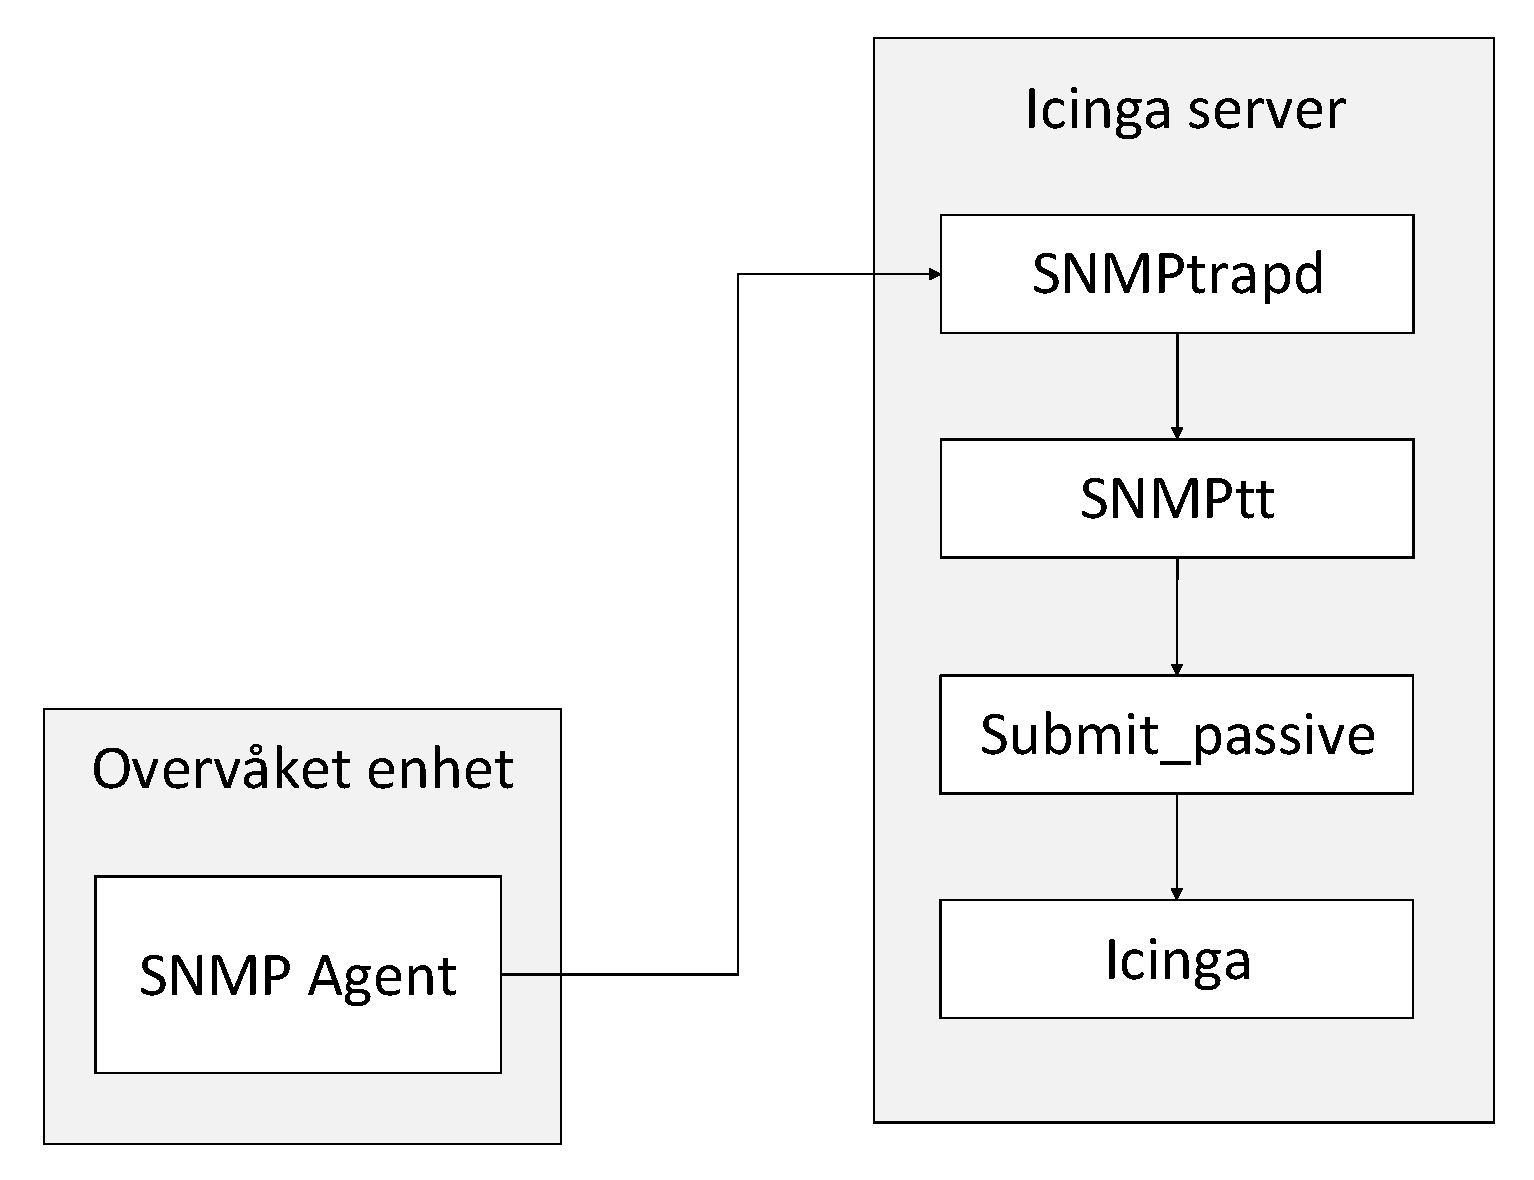
\includegraphics[scale=0.4]{img/SNMPtrap}
    \caption{Trap-prosessering}
    \label{snmptrap}
\end{figure}

SNMPtt trenger konfigurasjon for alle OID-ene som skal prosesseres. Disse kan opprettes med snmpttconvertmib ut i fra en MIB-fil slik:

\begin{lstlisting}[style=example]
root@icinga1:/usr/share/mibs/netsnmp# snmpttconvertmib --in=MERU-WLAN-MIB.my --out=meru.conf --exec='/usr/lib/nagios/plugins/libexec/submit_check_result "$aA meru_$N 2 $D"
\end{lstlisting}

Eksempel på en OID som blir generert i filen meru.conf:

\begin{lstlisting}[style=example]
EVENT mwlRogueApDetected .1.3.6.1.4.1.15983.3.1.3.13 "Status Events" Normal
FORMAT $*
EXEC /usr/lib/nagios/plugins/libexec/submit_check_result $aA meru_$N 2 "$D"
SDESC
A rogue AP is detected. The AP id, mac address, and other information are described in mwlTraContent.
EDESC
\end{lstlisting}

Her benyttes variabler i snmptt \cite{snmptrans}:
\begin{itemize}
	\item IP-adressen til snmp agenten, altså kontrollereren
	\item Navnet på trap-en
	\item Beskrivelse på trap fra konfigurasjonfilen.
\end{itemize}

SNMPtt vil så kjøre kommandoen definert under "EXEC" for OID-en, som i dette tilfellet er å sende informasjonen videre til scriptet "submit\_check\_result". Dette tar fire argumenter:

\begin{itemize}
	\item IP-adresse eller hostname 
	\item Service description
	\item Returkode som setter status på tjenesten (0-3)
	\item Plugin-output
\end{itemize}

Service description for alle meru traps som sendes inn vil da være "meru\_" + navnet på trap-en. Som plugin-output er det lagt inn beskrivelse av trap-en, da denne som regel er noe mindre kryptisk enn navnet.

Scriptet vil så skrive dette sammen med et timestamp til icinga.cmd som Icinga sjekker periodisk etter resultat av passive sjekker.

Noe å merke seg er at en ikke vil få informasjon når tjenesten er OK igjen, og må sette tjenestene til OK manuelt i Icingas webgrensesnitt.

\subsection{Serverrommiljø}
For å overvåke temperatur og luftfuktighet på serverrommet ble det kjøpt inn en APC NetBotz 200 \cite{netbotz2} med fire eksterne sensorer. Disse ble plassert slik at det er to sensorer på hver side av rack-raden. En vil dermed kunne se temperaturforskjellen mellom forsiden av serverne, ved luftinntak og baksiden, der varmluft går ut.

Hver sensor måler både temperatur og relativ luftfuktighet.

\subsubsection{Luftfuktighet}
Relativ luftfuktighet er definert som "forholdet mellom partielltrykket til vanndamp, i en gassblanding av luft og vann, og vanndampens metningstrykk ved en viss temperatur.". Dette gir en prosentandelen av vann i luften \cite{wiki:luftfuktighet}. 

Mange enheter for overvåkning av servermiljø måler også duggpunkt. Et duggpunkt er temperaturen en viss mengde luft må avkjøles til for at vanndamp skal kondensere. Ved en økning i relativ luftfuktighet vil duggpunktet nærme seg luftemperaturen. Ved 100 \% relativ luftfuktighet vil temperaturen og duggpunktet være like. 

I "Sun Microsystems Data Center Site Planning Guide" anbefales en luftfuktighet på 45 \% - 50 \%. Det meste av datautstyr kan fungere innenfor et bredere intervall enn det, typisk 20 \% - 80 \%. Men de anbefalte verdiene er satt for at det skal være et buffer dersom en har klimaanlegg som kontrollerer luftfuktighet, og det slutter å fungere \cite{planningserver}. Andre, som "American Society of Heating, Refrigerating and Air-Conditioning Engineers" (ASHRAE) anbefaler at den relative luftfuktigheten ikke bør overstige 60 \%, mens den nedre grensen er basert på duggpunkt og satt til 5.5° C, der den relative luftfuktigheten vil variere mellom 25 \% og 45 \% \cite{envguide}. Disse verdiene er også anbefalt av Cisco \cite{ciscoenvguide}, og omtalt som vidt akseptert. 

Høy luftfuktighet kan føre til kondens, som igjen kan føre til korrosjon på komponenter. Ved lavere luftfuktighet øker faren for utladninger av statisk elektrisitet (kritisk ved 30 \%), som kan føre til utladninger med ekstremt høye spenningsverdier. Dette kan ødelegge komponenter.

\subsubsection{Temperatur}
Det er mye uenighet rundt anbefalte verdier for temperatur i serverrom. I et studie utført ved University of Toronto \cite{torontopaper}, ble det samlet inn data fra tre forskjellige organisasjoners datasentre, deriblant Googles. I studiet ble det konkludert med at faren for hardware-feil ved høyere temperatur øker mindre enn det som har vært vanlig å basere seg på. For DRAM-feil og ``node outages'' fant de ingen korrelasjon til temperaturøkning for intervallet i testen (15° C - 60° C). I dette studiet ble det ikke målt eller tatt hensyn til luftfuktighet. 

ASHRAE anbefaler en inntakstemperatur 18° C - 27° C, mens Sun anbefaling er 20° C - 23° C. Sun begrunner sin anbefaling med at det er lettere å opprettholde trygge verdier for relativ luftfuktighet. ASHRAE refererer også til studier som viser at det totale strømforbruket kan gå opp ved høyere temperaturer, fordi enheter øker frekvensen på egne vifter \cite{datacentertemp}.

\subsubsection{Plugin for overvåkning av temperatur og luftfuktighet i Icinga}
Det fantes allerede en plugin for å sjekke sensorverdiene på APC NetBotz \cite{checknetbotz}. Men denne sammenlignet verdiene med grenseverdier satt i konfigurasjonen på enheten. Det var ønskelig å samle mest mulig av konfigurasjon på Icinga-serveren, derfor ble pluginen omskrevet til å kunne ta inn øvre og nedre grenseverdier som argumenter.

\subsection{UPS (Uninterruptible Power Supply)}
UPS, ofte kalt avbruddsfri strømforsyning på norsk, blir benyttet til å opprettholde strøm til alle enheter på IKT-avdelingens serverrom dersom strømnettet skulle falle ut. Strømmen filtreres også slik at utstyr ikke vil bli skadet av overspenning. Det beskytter derimot ikke mot overspenninger ved lynnedslag %TODO: /cite apc lynnedslag .

Ved IKT-avdelingen benyttes UPS-er av fabrikatene APC og HP.

For HP og APC overvåkes:
\begin{itemize}
 	\item Gjenstående batterikapasitet
	\item Prosentandel belastning
	\item Spenning inn og ut
	\item Temperatur (kun APC)
\end{itemize}

For både HP og APC overvåkes alle parametere direkte over SNMP med pluginen "check\_snmp" fra nagios-plugins. Her er OID-ene definert direkte i service-objektene.
